\documentclass[aps,pra, twocolumn]{revtex4-1}
\usepackage{amssymb,amsthm,amsmath,enumerate,url, natbib, graphicx, float, csvsimple, todonotes, enumitem}

\def\FCW{1.0\columnwidth}

\newcommand{\multi}[1]{\vec{#1}}
\newcommand{\bs}[1]{\boldsymbol{#1}}
\newcommand{\pr}{\mathrm{Pr}}
\newcommand{\pdiff}[2]{\frac{\partial #1}{\partial #2}}
\renewcommand{\d}{\mathrm{d}}
\newcommand{\M}{\mathcal{M}}
\newcommand{\R}{\mathcal{R}}
\newcommand{\Tr}{\mathrm{Tr}}
\newcommand{\Lik}{\mathcal{L}}
\renewcommand{\P}{\mathcal{P}}
\newcommand{\stup}{\uparrow}
\newcommand{\stdown}{\downarrow}
\newcommand{\stleft}{\leftarrow}
\newcommand{\stright}{\rightarrow}
\newcommand{\styplus}{\nearrow}
\newcommand{\styminus}{\swarrow}
\newcommand{\reals}{\mathbb{R}}
\newcommand{\cH}{\mathcal{H}}
\newcommand{\cL}{\mathcal{L}}
\newcommand{\Id}{\mathbb{I}}
\newcommand{\cI}{\mathcal{I}}
\newcommand{\ket}[1]{\ensuremath{\left|#1\right\rangle}}
\newcommand{\bra}[1]{\ensuremath{\left\langle\scriptstyle#1\right|}}
\newcommand{\braket}[2]{\ensuremath{\left\langle\scriptstyle#1|#2\right\rangle}}
\newcommand{\ketbra}[2]{\ket{#1}\!\!\bra{#2}}
\newcommand{\expect}[1]{\ensuremath{\left\langle#1\right\rangle}}
\newcommand{\braopket}[3]{\ensuremath{\bra{#1}#2\ket{#3}}}
\newcommand{\proj}[1]{\ketbra{#1}{#1}}
\newcommand{\union}{\cup}
\def\Id{1\!\mathrm{l}}
\newcommand{\Fi}{\mathcal{I}}

\newcommand{\bvec}[1]{\boldsymbol{#1}}
 

\newcommand{\rhohat}{\hat{\rho}}
\newcommand{\rhoBME}{\rhohat_{\scriptscriptstyle\mathrm{BME}}}
\newcommand{\rhoML}[1]{\rhohat_{\scriptscriptstyle{\mathrm{ML},#1}}}
\newcommand{\rhotomo}{\rhohat_{\scriptscriptstyle\mathrm{tomo}}}
\newcommand{\rhotrue}{\rho_{\scriptscriptstyle\mathrm{true}}}
\newcommand{\phat}{\hat{p}}

\newcommand{\diff}{\mathrm{d}\!}
\newcommand{\diffk}[1]{\mathrm{d}_{#1}\!}

\begin{document}
\author{Travis L Scholten}
\author{Robin Blume-Kohout}
\affiliation{Center for Computing Research (CCR), Sandia National Labs}
\affiliation{Center for Quantum Information and Control (CQuIC), University of New Mexico}

\title{Behavior of the Maximum Likelihood in Quantum State Tomography}

\begin{abstract}
Quantum state tomography on a $d$-dimensional system demands resources that grow rapidly with $d$. Model selection can be used to tailor the number of fit parameters to the data.  However, many methods rely on comparing test statistics (such as the ratio of two models' maximum likelihoods) to their expected behavior under baseline assumptions.  In state tomography, the presence of positivity constraints (e.g. $\rho\geq0$) can violate those assumptions, especially local asymptotic normality.  Applying those methods to state tomography thus requires understanding and quantifying how positivity constraints affect test statistics.  Here, we study the behavior of the maximum likelihood in different Hilbert space dimensions, and derive an expression for the expected value of the loglikelihood ratio statistic (roughly, the logarithm of the maximum likelihood) between  state spaces of different Hilbert space dimension $d$.  In addition to enabling reliable model selection, our results shed more light on qualitative effect of positivity constraints on state tomography.
\end{abstract}
\date{\today}

\maketitle


\todo{I hate that phrase. Need a new one} In quantum information science, an experimentalist may wish to determine the quantum state $\rho_{0}$ that is produced by a specific initialization procedure.  This can be done using quantum state tomography \cite{Paris2004}:  many copies of $\rho_{0}$ are produced; they are measured in diverse ways; and finally the outcomes of those measurements (data) are collated and analyzed to produce an estimate $\rhohat$.  This is a straightforward statistical inference process \cite{Reid2015, Wasserman2004}, where the data are used to fit the parameters of a statistical model.  However, we don't always know what model to use.  In state tomography, the parameter is $\rho$, and the model is the set of all possible density matrices on a Hilbert space $\cH$ (equipped with the Born rule). It is not always \emph{a priori} obvious what $\cH$ or its dimension is; examples include optical modes \cite{Altepeter2005, Bertrand1987, Lvovsky2009, Breitenbach1997, Leonhardt1995} and leakage levels in AMO and superconducting \cite{Motzoi2009, Fazio1999} qubits. In such situations, we seek to let the data itself determine which of many candidate Hilbert spaces is best suited for reconstructing $\rho_{0}$.

Choosing an appropriate Hilbert space on the fly is an instance of a general statistical problem called \emph{model selection}.  Although model selection has been thoroughly explored in classical statistics \cite{Burnham2004}, its application to quantum tomography encounters some obstacles.  They stem from the fact that quantum states (and thus, estimates of them) must satisfy a \emph{positivity constraint} ($\rho\geq0$).  A similar constraint (complete positivity) applies to process tomography.  The impact of positivity constraints on state and process tomography is an active area of research \cite{Candes2006, Flammia2012a, Suess2016, Carpentier2015}, and its implications for model selection have also been considered \cite{Schwarz2013a, Guta2012a, VanEnk2013a, Langford2013, Yin2011, Moroder2013, Knips2015}.  In this paper, we address a specific question at the heart of this matter:  \emph{How does the loglikelihood ratio statistic used in many model selection protocols, including (but not limited to) information criteria such as Akaike's AIC, \todo{ref?}behave in the presence of the positivity constraint $\rho\geq0$?}  We begin by introducing $\lambda$, the loglikelihood ratio statistic, and outlining how it can be used to choose a Hilbert space dimension.  Then, we show how and why the standard model of its behavior, the Wilks theorem, falls apart in the presence of positivity constraints.  We propose a new theory that explicitly accounts for state space boundaries, and we derive a closed-form approximation for $\lambda$'s expected value under the same conditions as the Wilks theorem -- but \emph{with} the $\rho\geq0$ constraint.  Finally, we test the validity of our approximate theory under harsh conditions by comparing it to numerical results for the realistic problem of optical heterodyne tomography.

\todo[inline]{Is there some figure we could draw here?}

\section{Introduction - Statistical Model Selection}

Discussing model selection for state tomography requires introducing some basic statistical notions.  A \emph{model} is a parameterized family of probability distributions over some data $D$, usually denoted as $\mathrm{Pr}_{\bs{\theta}}(D)$, where $\bs{\theta}$ are the \emph{parameters} in the model. In quantum state tomography, the data are the outcomes of the measurements of a positive operator-valued measure (POVM) $\{E_{j}\}$, the parameters are a quantum state $\rho$, and the probability of obtaining outcome ``$j$" is given by the Born rule: $p_{j} = \mathrm{Tr}(\rho E_{j})$ \footnote{The index $j$ may be continuous or discrete.}. In this paper, a model is a set of density matrices, and $\rho$ indicates a particular choice of the model's parameters.

Suppose we have some data obtained from an unknown state $\rho_{0}$, and two candidate models $\M_{1}, \M_{2}$ that could be used to fit it.  Many of the known methods for choosing between them (i.e., model selection) involve quantifying how well each model fits the data by its \emph{likelihood}.  The likelihood of a simple hypothesis $\rho$ is defined as $\mathcal{L}(\rho) = \mathrm{Pr}(\mathrm{Data}|\rho)$.  Models, however, are \emph{composite} hypotheses, comprising many possible values of $\rho$.  A canonical way to define model $\M$'s likelihood is via the general method of \emph{maximum likelihood} (ML), by maximizing $\cL(\rho)$ over $\rho\in\M$.  In practice, the maximization is usually done explicitly to find an ML estimate $\hat{\rho}_{\mathrm{ML},\M}$ \cite{Hradil1997, JamesPRA2001, Blume-Kohout2010} of $\M$'s parameters, and then $\cL(\M) = \cL(\hat{\rho}_{\mathrm{ML},\M})$.  (Note: although it is common to refer to $\hat\rho_{\mathrm{ML}}$ without specifying the model over which $\cL$ was maximized, we list the model explicitly in the subscript because in this paper we are constantly maximizing over different models!)

Within this framework, models can be compared using the \emph{loglikelihood ratio} \cite{Neyman1933, Blume-Kohout2010, Moroder2013}:
\begin{align}
\lambda(\M_{1}, \M_{2}) &= -2 \log \left(\frac{\cL(\M_{1})}{\cL(\M_{2})}\right)\\
&= -2 \log \left(\frac{\cL(\rhoML{\M_{1}})}{\cL(\rhoML{\M_{2}})}\right)\\
&= -2 \log \left(\frac{\underset{\rho \in \M_{1}}{\max}~\cL(\rho)}{\underset{\rho \in \M_{2}}{\max}~\cL(\rho)}\right).
\end{align}
All else being equal, a positive $\lambda$ favors $\M_2$ -- i.e., the model with the higher likelihood is more plausible, because it fits the data better.  However, all else is rarely equal.  If both models are equally valid -- e.g. they both contain $\rho_0$ -- but $\M_2$ has more parameters, then $\M_2$ will very probably fit the data better.  Models with more adjustable parameters do a better job of fitting \emph{noise} (e.g. finite sample fluctuations) in the data.  This becomes strictly true when the models are \emph{nested}, so that $\M_{1} \subset \M_{2}$.  In this case, the maximum likelihood of $\M_{2}$ is at least as high as that of $\M_{1}$.  Not only is $\lambda \geq 0$, but almost surely $\lambda > 0$.  Remarkably, the same effect also makes $\M_{2}$'s fit less accurate (almost surely), because that fit incorporates more of the noise in the data.  These two effects constitute \emph{overfitting}, which can be summed up as ``Extra parameters make the fit look better, but perform worse.''  This provides strong motivation to correct for overfitting by handicapping larger models, to prevent them from being chosen over smaller models that are no less valid, and may even yield better estimates in practice \cite{Akaike1974}.

For this reason, any model selection method that relies (explicitly or implicitly) on a statistic to quantify ``how well model $\M$ fits the data'' also relies on a \emph{null theory} to predict how that statistic will behave if $\rho_{0} \in \M$.  A model selection criterion based on an invalid null theory (or a criterion used in a context where its null theory does not apply) will tend to choose the wrong model.

The null theory may be used to formulate a \emph{decision rule} for choosing between two models. By knowing how the statistic behaves when both models are equally good, we may then compare the observed value of the statistic to the null theory. If the observed value is very improbable under the null theory, then that constitutes evidence against the smaller model, and justifies rejecting it. On the other hand, if the observed value is \emph{consistent} with the null theory, there is no reason to reject the smaller model.

The standard null theory for $\lambda$, the \emph{Wilks theorem} \cite{Wilks1938}, relies on \emph{local asymptotic normality} (LAN) \cite{LeCam1970, LeCam1956}. LAN means that: (1) as $N_{\mathrm{samples}}\rightarrow \infty$,  $\rhohat_{\mathrm{ML}}$ is normally distributed around $\rho_{0}$ with covariance matrix $\Fi^{-1}$, and (2) the likelihood function in a neighborhood of $\rhohat_{\mathrm{ML}}$ is locally Gaussian with Hessian $\Fi$, where $\Fi$ is the classical \emph{Fisher information matrix} associated with the POVM. It quantifies how much information the data carries about a parameter in the model. Generally speaking, the Fisher information depends strongly on $\rho_{0}$ and the POVM being measured.

Most statistical models satisfy LAN.  When LAN holds \emph{and} the number of samples is large enough to reach the ``asymptotic" regime, the Wilks theorem states that if $\rho_{0}\in \M_{1}\subset \M_{2}$, where $\M_{1}$ has $k$ free parameters and $\M_{2}$ has $K+k$ free parameters, then $\lambda$ is a $\chi^{2}_{K}$ random variable.  This is a complete null theory for $\lambda$ (under the specified conditions), and implies that $\langle \lambda \rangle = K$ and $\Delta \lambda = \sqrt{2K}$.

Therefore, in the ``Wilks regime", a simple rule for model selection would be the following: compare the observed value of $\lambda$ to $\lambda_{\mathrm{thresh}} = \langle \lambda \rangle + n\Delta \lambda$, for some $n \approx 1$, and reject the smaller model if $\lambda > \lambda_{\mathrm{thresh}}$.  While model selection rules can be more subtle and complex than this \todo{Think about citations here, somewhat carefully}, they usually take the general form of a threshold in which $\expect{\lambda}$ plays a key role.  Rather than attempting to define a specific rule, our focus in this paper is to understand the behavior of $\expect{\lambda}$ and derive an approximate expression for it in the context of state tomography.

The first step in doing so is to explain how, and why, the Wilks theorem can break down for state tomography.

\begin{figure}[h]
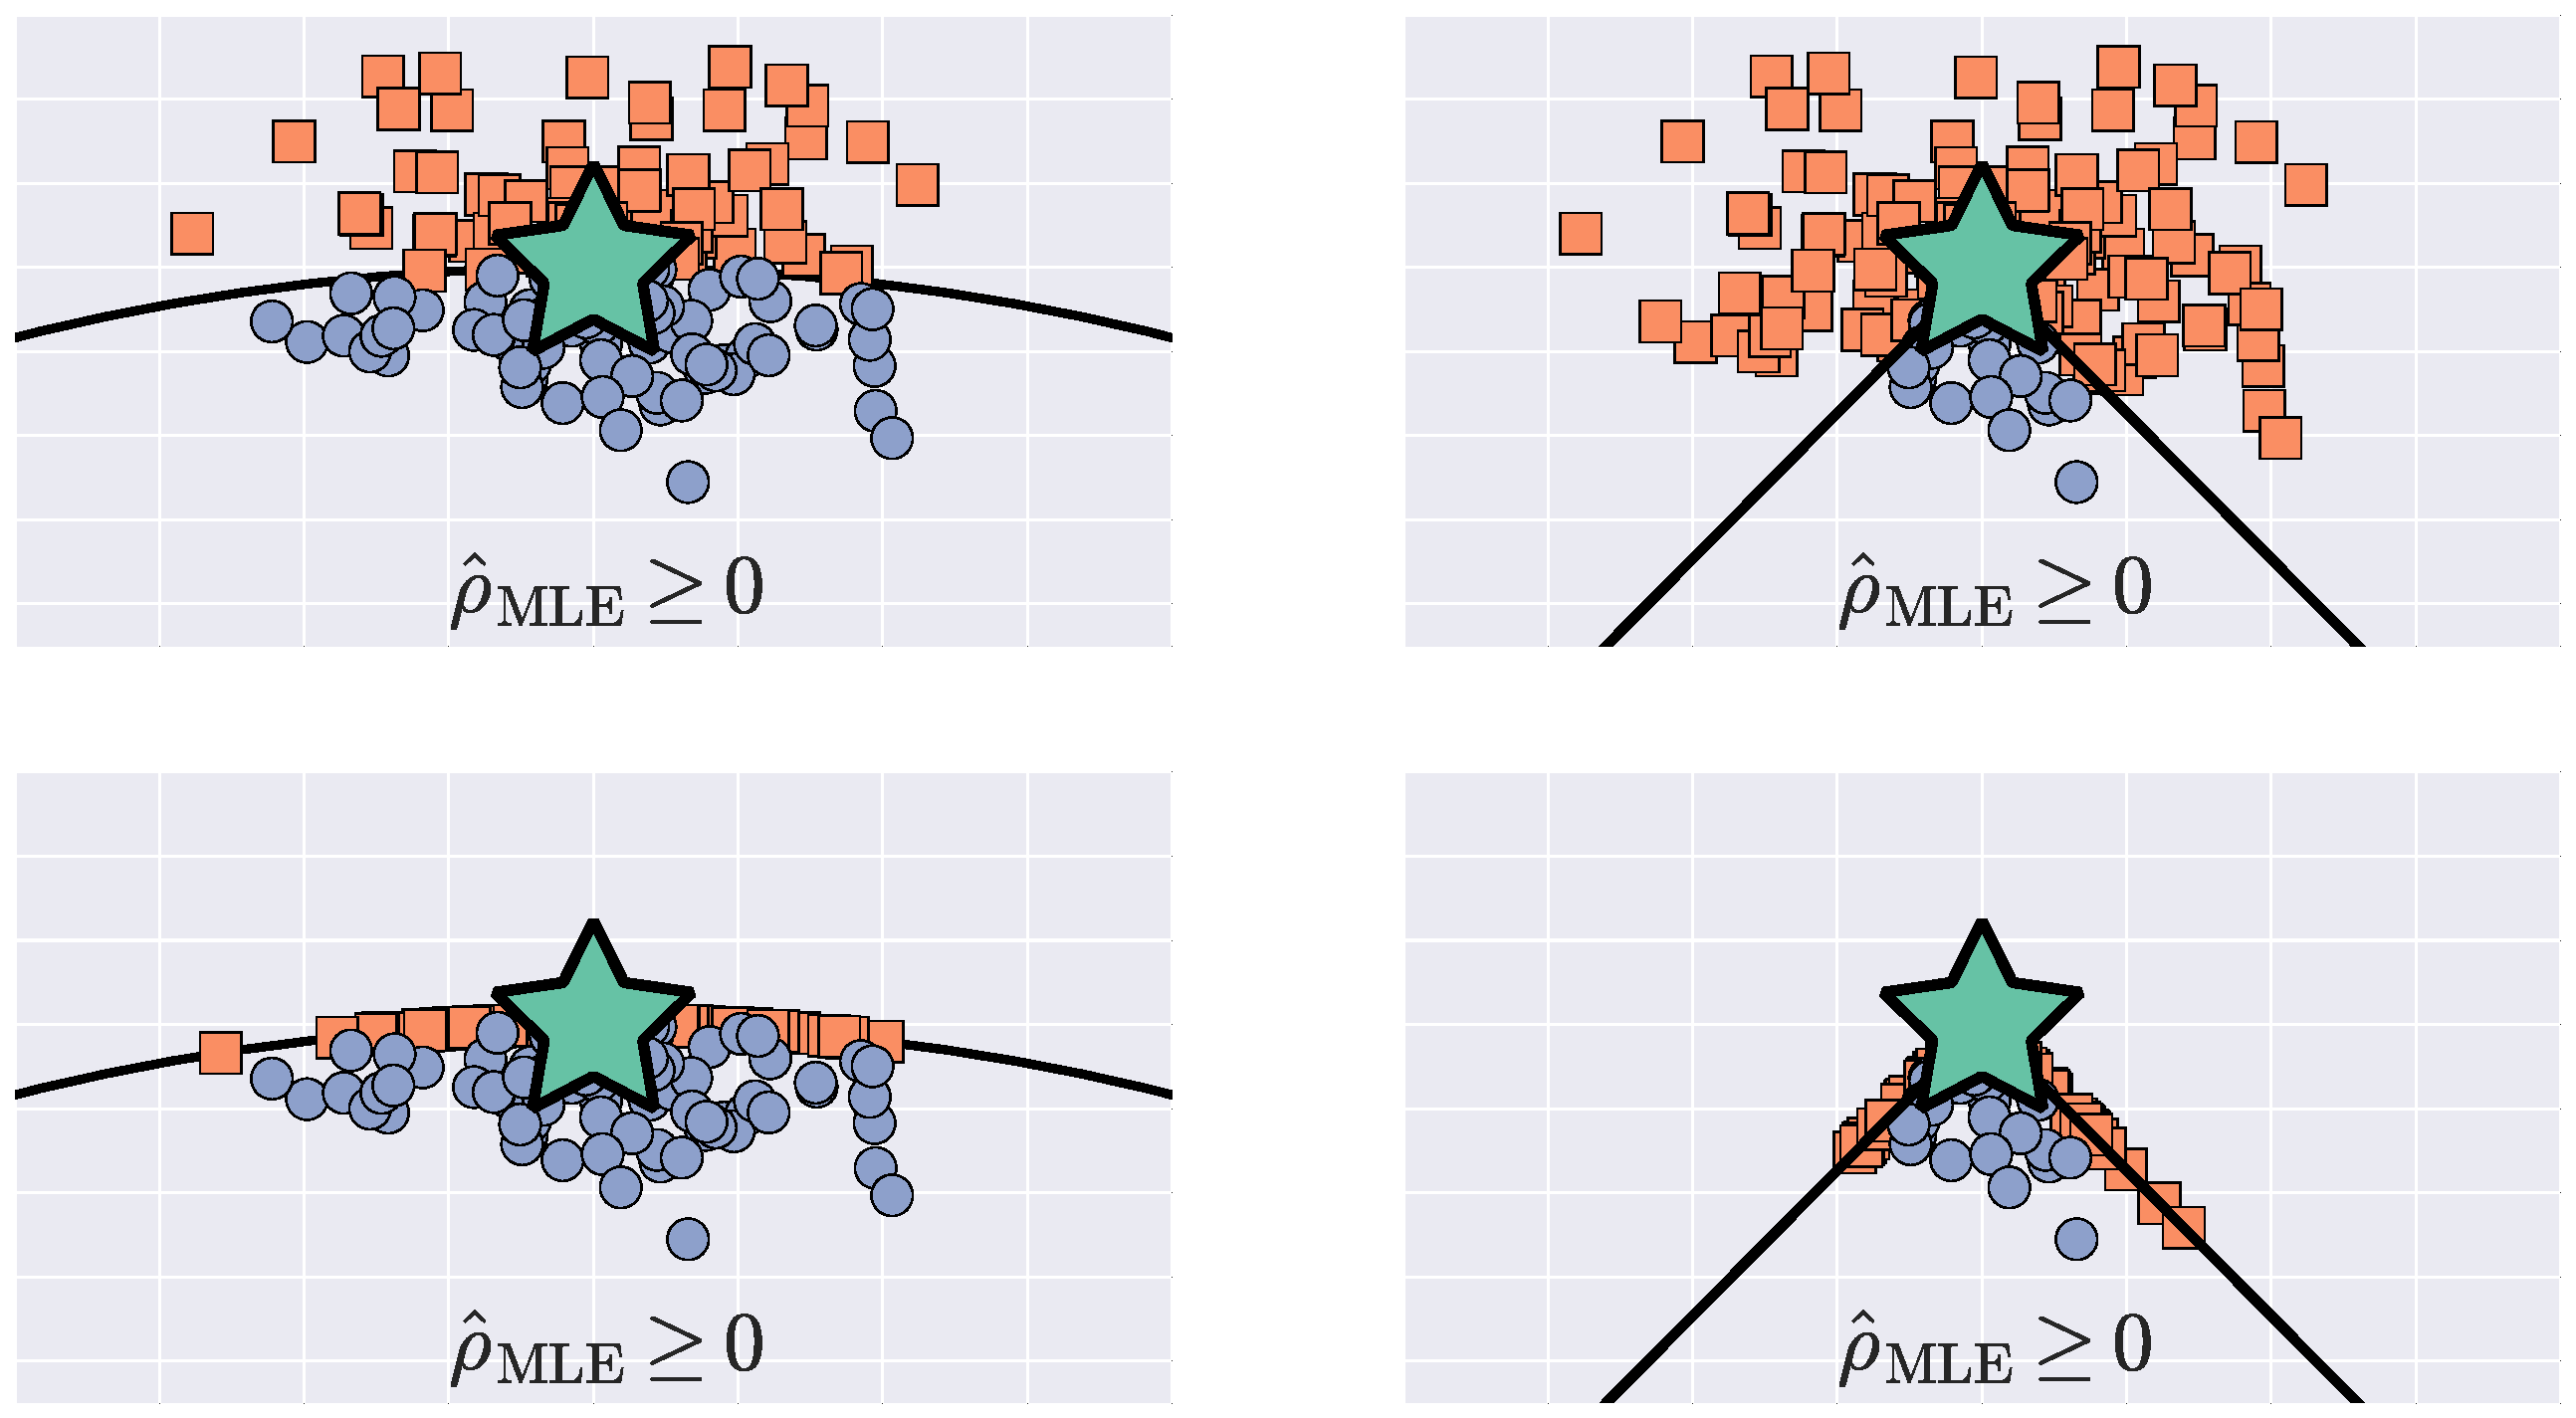
\includegraphics[width=\columnwidth]{Images/Figure_1.pdf}
 \caption{Impact of the boundary on maximum likelihood tomography. \textbf{Top}: Two views through the qutrit state space. Without the positivity constraint, some estimates (orange squares) are not positive semidefinite, and do not represent valid estimates of a quantum state. The distribution of $\rhoML{3}$ (blue circles) is generally non-normal, and depends on the true state $\rho_{0}$ (star).
\textbf{Bottom}:  Comparison of the classical theory (Wilks theorem) prediction for the loglikelihood ratio $\expect{\lambda}$ to numerical data for states $\rho_{0}$ with ranks $r=1,\ldots ,10$.  The Wilks theorem fails badly for low-rank states; our main result (Equation \ref{eq:ourLLRS}) fixes this problem (see Figure \ref{fig:modelcomp-iso}).}
\label{fig:boundaries}
\end{figure}

\section{Quantum State Tomography and Model Selection}

Quantum state tomography typically begins with $N$ independently and identically prepared quantum systems -- i.e., $N$ copies of an unknown state $\rho_{0}$.  Each copy is measured, and without loss of generality \todo{This isn't obvious to me}we can assume that each measurement is described by the same positive operator-valued measure (POVM).  A POVM is a collection of positive operators $\{E_j\}$ summing to $\Id$, and the probability of outcome ``$j$'' is given by $\Tr(\rho_0 E_j)$.  The results of all $N$ measurements constitute data:  a record of the various possible outcomes' frequencies $\{n_{j}\}$, where $n_{j}$ is the number of times ``$j$'' was observed, and $\sum_{j}n_{j} = N$.  Finally, this data is processed through some \emph{estimator} to yield an estimate $\hat{\rho}$ of $\rho_0$.  A variety of estimators have been proposed \cite{Vogel1989,Hradil1997,JamesPRA2001,Blume-Kohout2010b,Blume-Kohout2010,Zhu2014a,Ferrie2016}, but this is not our concern here.  However, since we \emph{are} concerned with computing the likelihood of a model $\M$, which is defined as likelihood of the most likely $\rho\in\M$, we will make extensive use of the \emph{maximum likelihood} (ML) estimator $\rhoML{\M}$.  This should not be taken as advocacy for the ML estimate; it is only a convenient way to find the maximum of $\cL$ over $\M$ as $\mathcal{L}(\rhoML{\M})$, and once a model is chosen, a different estimator could be used.

The likelihood $\mathcal{L}(\rho)$ is
\begin{equation}
\mathcal{L}(\rho) = \prod_{j}\mathrm{Tr}(\rho E_{j})^{n_{j}},
\end{equation}
so $\rhoML{\M}$ is the solution to the optimization problem
\begin{equation}
\rhoML{\M} = \underset{\rho \in \M}{\text{argmax}}~\mathcal{L}(\rho).
\end{equation}
In state tomography, $\M$ is almost always the set of all density matrices over a Hilbert space $\cH$:
\begin{equation}
\mathcal{M}_{\cH} = \{\rho~|~\rho \in \mathcal{B}(\mathcal{H}),~\mathrm{Tr}(\rho) =1,~\rho \geq 0\},
\end{equation}
where $\mathcal{B}(\cH)$ is the space of bounded (linear) operators on $\cH$.  To solve the optimization problem, we can use the following facts: (a) $\M_{\cH}$ is a convex set, and (b) $\rhoML{\M}$ also maximizes the value of $\log(\cL(\rho))$, which is a convex function. Because $\rhoML{\M}$ is the solution to an optimization problem involving a convex function defined over a convex set, it can be found efficiently via any of several algorithms for convex optimization \cite{Boyd}.

Usually, $\cH$ is taken for granted or chosen by fiat.  In this paper, we will consider a nested family of different Hilbert spaces, indexed by their dimension $d$: $\cH_{1}  \subset \cdots \subset \cH_{d} \subset \cH_{d+1} \subset \cdots$.  The models we consider are therefore given by:
\begin{equation}
\M_{d} \equiv \mathcal{M}_{\cH_{d}} = \{\rho~|~\rho \in \mathcal{B}(\mathcal{H}_{d}),~\mathrm{Tr}(\rho) =1,~\rho \geq 0\}.
\end{equation}
To select between these models, we need to determine whether one model (say, $\M_{d + 1}$) is ``better'' than another (say, $\M_{d}$).  To evaluate which is better, we typically fit both models to the data, and see how well those fits perform (as measured by some notion of ``goodness of fit"). However, this implies that in our pursuit of finding the best model, we would naively end up choosing a model with highest value of $\cL(\M)$. Although fitting the data is an important consideration in evaluating the goodness of a model, we need to avoid \emph{overfitting}, a situation in which the model fits the data extremely well, but is not able to accurately predict anything about \emph{future} data. To avoid choosing a model which would overfit the data, it is necessary to penalize or handicap larger models, since (all else being equal) they will \emph{always} fit the data better.  Doing so requires a null theory predicting how our test statistic -- $\lambda(\M_{d}, \M_{d+1})$, the loglikelihood ratio between $\M_d$ and $\M_{d+1}$ -- behaves when both models are valid, i.e. when $\rho_{0} \in \M_{d},\M_{d + 1}$.

In classical statistics, the null theory for $\lambda$ (the Wilks theorem) relies on local asymptotic normality (LAN).  If LAN holds, the likelihood function near $\rhohat_{\mathrm{ML}}$ is given by
\begin{equation}
\mathcal{L}(\rho) \propto \text{Exp}\left[-(\rho - \rhohat_{\mathrm{ML}})\mathcal{I}(\rho - \rhohat_{\mathrm{ML}})/2\right],
\end{equation}
and the distribution of $\rhohat_{\mathrm{ML}}$ is
\begin{equation}
\mathrm{Pr}(\rhohat_{\mathrm{ML}}) \propto \text{Exp}\left[-(\rho_{0} - \rhohat_{\mathrm{ML}})\mathcal{I}(\rho_{0} - \rhohat_{\mathrm{ML}})/2\right],
\end{equation}
where $\mathcal{I}$ is the \emph{Fisher information matrix}.  (Note that in expressions involving $\mathcal{I}$, states $\rho$ are treated as vectors in state space, and $\mathcal{I}$ is a matrix or 2-index tensor acting on that state space).  In classical statistics, it is common to assume that boundaries are not relevant, either because the models of interest have none, or by assuming that the true parameter values $\rho_{0}$ lie far away from them.  In the absence of boundaries, and in the asymptotic limit where curvature of the Fisher metric is also negligible, many statistics calculations can be simplified by changing to \emph{Fisher-adjusted} coordinates in which the Fisher information is isotropic (i.e., $\mathcal{I}\propto\Id$).
\todo{Write out that transformation?}

But the statistical models used for quantum state tomography \emph{do} have boundaries.  When $\rho_{0}\in \M_{d}$ and has rank $r = d$, LAN will hold -- which is to say that, asymptotically, the boundary can indeed be ignored.  In that case, the Wilks theorem applies, and $\lambda(\M_{d}, \M_{d + 1}) \sim \chi^{2}_{2d + 1}$.  But when $\rho_{0}$ has rank $r<d$, it lies \emph{on} the boundary of the model (see Figure \ref{fig:boundaries}).  LAN does not hold, because even asymptotically, positivity constrains $\rhoML{d}$, and so $\mathrm{Pr}(\rhoML{d})$ is not Gaussian.  The Wilks theorem does not apply in this case.  Moreover, this is the relevant situation for our analysis, because \emph{even if $\rho_{0}$ is full-rank in $\M_{d}$, it must be rank-deficient in $\M_{d+1}$}.  So we are forced to derive a replacement for the Wilks theorem, a null theory for $\lambda$ when $\rho_0$ is rank-deficient.

The distributions of $\rhoML{d}, \rhoML{d+1}$ are complicated, highly non-Gaussian, and singular (because estimates ``pile up'' on the various faces of the boundary).  For this reason, we will not attempt to compute $\mathrm{Pr}(\lambda)$ directly.  Instead, we focus on deriving a good approximation for $\langle \lambda \rangle$.

Furthermore, the Fisher information $\mathcal{I}$ is generally anisotropic. \todo{See Figure ??} And while the constraint $\rho\geq0$ that invalidates LAN in the first place is at least somewhat tractable in standard (Hilbert-Schmidt) coordinates, it becomes completely intractable in Fisher-adjusted coordinates.  So, to obtain a semi-analytic null theory for $\lambda$, we will make the simplifying assumption that $\mathcal{I}$ is proportional to the Hilbert-Schmidt metric ($\mathcal{I} \propto \Id$).

The main section of this paper is devoted to approximating $\expect{\lambda}$ under the assumption $\mathcal{I} \propto \Id$; the main result is given in Equation \eqref{eq:ourLLRS}.  Then, in the last section of the paper, we check the robustness of the results that we derive with this simplifying assumption, by performing a numerical study of a tomography problem where $\mathcal{I}$ is \emph{extremely} anisotropic and comparing the results to the predictions derived with $\mathcal{I} \propto \Id$.

\missingfigure{Picture of $\rhohat$, $\hat{\rho}_{\mathrm{ML}}$, etc. w/ anisotropic Fisher information}

\section{Deriving a Replacement for the Wilks theorem}

In this section, we show how to derive a replacement for the Wilks theorem which is valid for rank-deficient $\rho_{0}$. To do so, we provide a replacement for LAN in the presence of boundaries, which we call \emph{Local Asymptotic Metric-Projected Normality} (LAMPN). The choice of name for this property comes from the fact that we borrow terminology and ideas from convex optimization and compressed sensing. Briefly, LAMPN is a property of our constrained statistical model $\M_{d}$, under the following assumptions:

\begin{itemize}
\item $\M_{d}$ may be written as a subset of a larger, unconstrained model $\M'$.
\item For each point $\rho_{0} \in \M_{d}$ (the ``true state"), LAN holds in $\M'$.
\end{itemize}

In state tomography, $\M'$ is the set of all trace-1, Hermitian matrices. (That is, a matrix $\hat{\rho} \in \M'$ need not satisfy $\hat{\rho} \geq 0$.) Each $\hat{\rho} \in \M'$ is an \emph{unconstrained} MLE, and LAN holds.

With these two assumptions, it's possible to show that, asymptotically, the \emph{local state space} around $\rho_{0}$ converges to its \emph{tangent cone}. In turn, this implies the distribution of MLEs we would obtain by maximizing the likelihood in Equation ?? is the same as that which we would obtain by taking an \emph{unconstrained} distribution, and projecting them onto the tangent cone.

The reason for using ``metric-projected normality", as opposed to ``projected normality", is because in the convex optimization community, the phrase ``metric projection" is used to denote the vector $\Pi_{C}(\bs{x})$ that is the projection of $\bs{x}$ onto a cone $C$ (and where the metric defining the projection is Euclidean):
\[\Pi_{C}(\bs{x}) = \underset{\bs{y}\in C}{\text{argmin}}~||\bs{x}  -\bs{y}||^{2}\]
\todo[inline]{citation?}
There's a clear connection between metric projections and MLEs over $\M_{d}$; namely, $\rhoML{d}$ is simply the metric projection of $\sigma$ onto $M_{d}$!
\[\rhoML{d} = \underset{\rho \in \M_{d}}{\text{argmin}}~||\rho  -\hat{\rho}||^{2}\]
\todo[inline]{More clear explanation}

The exact behavior of $\rhoML{d}$, and $\lambda(\M_{d}, \M_{d+1})$ is complicated; however, by assuming $N_{\mathrm{samples}} \rightarrow \infty$, it's possible to replace projecting $\sigma$ onto $\M_{d}$ with projecting it onto the \emph{tangent cone} at $\rho_{0}$, $T(\rho_{0})$:
\[\rhoML{d} = \underset{\rho \in T(\rho_{0})}{\text{argmin}}~||\rho  -\hat{\rho}||^{2}\]
What's more, it's possible to derive an exact expression for $\lambda(\M_{d}, \M_{d+1})$:
\[\lambda(\M_{d}, \M_{d+1}) = \mathrm{Tr}[(\rho_{0} - \rhoML{d+1})^{2}] -  \mathrm{Tr}[(\rho_{0} - \rhoML{d})^{2}] \]



\todo[inline]{Something about $\lambda$ being equal to (scaled) mean-squared error.}




\subsection{Technical Details}

\subsubsection{Defining LAMPN}

In this section, we provide the technical details and proofs omitted in the previous section. To set up the problem, we consider a constrained statistical model $\M$, and assume $\M \subset \M'$, where $\M'$ is an \emph{unconstrained} model. Further, we assume that for each $\rho_{0} \in \M$, LAN holds in $\M'$. As LAN is an asymptotic property of the model $\M'$, all of our results will be derived in the $N \rightarrow \infty$ limit.

Consider a $\rho_{0} \in \M$ such that LAN holds in $\M'$. Letting $\hat{\rho}$ denote the ML estimate in $\M'$, as $N \rightarrow \infty$,
\[\mathrm{Pr}(\hat{\rho})\xrightarrow[]{\text{d}} \mathcal{N}\left(\rho_{0}, \Sigma\right)\]
where $\xrightarrow[]{\text{d}}$ means ``converges in distribution to", and $\Sigma$ is the \emph{covariance matrix} of the MLEs. Above, we assumed $\Sigma \propto \Id$; in what follows, we assume $\Sigma = \Id/N$.

Suppose we draw a closed ball $\mathcal{B}$ around $\rho_{0}$, whose radius is $N^{-1/4}$:
\[\mathcal{B}(\rho_{0}, N) =\{\rho~|~||\rho - \rho_{0}||_{2} \leq 1/N^{1/4}\}\]

It turns out that, asymptotically, $\mathcal{B}$ contains all the MLEs:
 \[\lim_{N \rightarrow \infty}\left[\mathrm{Pr}\left(\hat{\rho} \in \mathcal{B}\right)\right] \rightarrow 1\]

Showing this requires doing a few integrals:
\begin{align*}
\end{align*}
\todo[inline]{Um....?}
 
Further, we observe that $\M_{d}$ has a finite \emph{diameter} and in turn, a finite \emph{radius} $R$. Independent of $d$, the diameter of quantum state space is $2$ (consider the Hilbert-Schmidt distance between $\rho$ and $\sigma$, where $\rho$ and $\sigma$ are orthogonal pure states.

 To summarize, in Hilbert-Schmidt coordinates, we have
 
 \begin{itemize}
 \item $\Sigma = \Id/N$
 \item $\mathcal{B}$ has a radius $1/N^{1/4}$
 \item $\M_{d}$ has radius $1$
 \item $\mathrm{Pr}\left(\hat{\rho} \in \mathcal{B}\right) = 1$, asymptotically.
 \end{itemize}
 
Now, we switch to \emph{Fisher-adjusted} coordinates, so that the covariance matrix of the MLEs is equal to the identity, not just proportional to it. This coordinate transformation may be obtained simply by sending $\rho \rightarrow N^{1/2}\rho$.

This transformation then changes the covariance matrix of the MLEs, because for any random variable $\bs{x}$,
\[\mathrm{Cov}(A\bs{x}) = A\mathrm{Cov}(\bs{x})A^{T} \]
for any $A$. Choosing $A = N^{1/2}\Id$ gives
\[\mathrm{Cov}(N^{1/2}\Id\hat{\rho}) = \Id\]

 Thus, in Fisher-adjusted coordinates, the covariance matrix of the MLEs is the identity.

Further, the radius of the state space changes, because the diameter is enlarged, due to the fact that distances are rescaled:
\[||\rho - \sigma||^{2} \rightarrow N||\rho - \sigma||^{2}\]
Therefore, the diameter and radius of the state space are each increased by a factor of $N^{1/2}$. In turn, this implies the radius of $\mathcal{B}$ is increased to $N^{1/2}*N^{-1/4} = N^{1/4}$.
\todo[inline]{Show that Pr MLE in ellipsoid still 1}

In Fisher-adjusted coordinates, we have

 \begin{itemize}
 \item $\Sigma = \Id$
 \item $\mathcal{B}$ has radius $N^{1/4}$
 \item $\M_{d}$ has radius $\sqrt{N}$.
 \item $\mathrm{Pr}\left(\hat{\rho} \in \mathcal{B}\right)$ approaches 1, asymptotically.
 \end{itemize}

Finally, we translate the entire inference problem by establishing $\rho_{0}$ as the \emph{origin} of our parameter space. (That is, we send $\rho \rightarrow \rho - \rho_{0}$.) Because translation doesn't change Euclidean distance, all the properties above still hold in this new coordinate system.

By going to these coordinates, we are able to prove a useful result about the geometry of the region contained in the intersection of the state space and $\mathcal{B}$ --  the \emph{local state space} converges to a \emph{tangent cone}. Tangent cones are a general feature of points on the surface of convex sets (see \cite{Rockafellar1998}, Chapter 6, Section A), and are defined as follows:

\textbf{Definition: Tangent Cone} 
For each point $X$ on a convex surface $S$, the tangent cone $T(X)$ is defined as the following limit:
\[T(X) = \lim_{N\rightarrow \infty} S_{N}\]
where $S_{N}$ is a \emph{homothetic transformation} of $S$ with respect to $X$, with homothety coefficient $N$:
\[S_{N} = \{X + NY  |~\forall ~Y \neq X \in S\}\]

Under this definition, the tangent cone naturally arises as the limit of surfaces formed by fixing $X$, and then scaling up every other point on the surface with respect to it. ($X$ itself is known as the \emph{homothetic center} of the tangent cone.) Such a picture naturally arises in the context of LAMPN, as we are interested in what the local state space looks like as the distribution of unconstrained MLEs becomes more and more tightly concentrated around $\rho_{0}$.

In the asymptotic limit, the behavior of the MLEs is entirely determined by their behavior within $\mathcal{B}$, as it contains almost all of them. Further, in Fisher-adjusted coordinates, as $N\rightarrow \infty$, both the ball and the state space expand, but at different rates. Because the state space expands at a faster rate than the ball, it can never be the case that $\M_{d}\subset \mathcal{B}$, meaning there is always some part of the state space we are ignoring. That's acceptable, as we are interested in the \emph{local asymptotic} behavior of the MLEs.

To complete the proof, we define the surface $S_{N}$ as the surface of the intersection of $\M_{d}$ and $\mathcal{B}$:
\[S_{N} = \text{Surface}(\M_{d} \cap \mathcal{B}(\rho_{0}, N))\]
If $\rho_{0}$ is rank-deficient within $\M_{d}$, then $S_{N}$ is a genuine surface. \todo{what does that even mean?}. Considering $N \rightarrow \infty$, $S_{N}$ will converge to the tangent cone at $\rho_{0}$, $T(\rho_{0})$. However, if $\mathrm{Rank}(\rho)  = d$, then $S_{N}$ will converge to $\mathbb{R}^{d^{2}-1}$.\todo{this isn't clear}

\subsubsection{Expression for $\lambda(\M_{d}, \M_{d+1})$}

In comparing any two models using the loglikelihood ratio statistic, it's possible to do so by comparing each to any \emph{reference model} $\M$. Here, we take $\M = \rho_{0}$:
\[\lambda(\M_{d}, \M_{d+1}) = \lambda(\rho_{0},\M_{d+1}) - \lambda(\rho_{0},\M_{d})\]
Under the assumption of LAMPN, $\lambda(\rho_{0}, \M_{d})$ has a simple form. This follows from the fact that under this assumption
\[\rhoML{d} = \underset{\rho \in T(\rho_{0})}{\text{argmin}}~||\rho  -\hat{\rho}||^{2}.\]
and
\begin{equation}
\label{eq:tangentLLRS}
\lambda(\rho_{0}, \M_{d}) = \mathrm{Tr}[(\rho_{0} -\hat{\rho})^{2}] -   \mathrm{Tr}[(\rhoML{d} - \hat{\rho})^{2}]
\end{equation}

\textbf{Lemma:}

Under LAMPN, $\lambda(\rho_{0}, \M_{d}) = \mathrm{Tr}[(\rho_{0} - \rhoML{d})^{2}]$.

\textbf{Proof:}

\emph{Case 1}: Assume $\hat{\rho} \not \in T$. Because $\rhoML{d}$ is the closest point to $\hat{\rho}$ in $T$, and because $T$ contains $\rho_{0}$ (the origin), the lines joining $\rho_{0}$ to $\rhoML{d}$, and $\rhoML{d}$ to $\hat{\rho}$, are at right angles to one another. (See Figure ??) Applying the Pythagorean theorem, we have
\begin{equation}
\label{eq:pythag}
\mathrm{Tr}[(\rho_{0} -\hat{\rho})^{2}] =  \mathrm{Tr}[(\rho_{0} - \rhoML{d})^{2}] + \mathrm{Tr}[(\rhoML{d} - \hat{\rho})^{2}]
\end{equation}
Doing a subtraction, and comparing with Equation \eqref{eq:tangentLLRS}, yields the result.

\emph{Case 2}: Assume $\hat{\rho} \in T$. Then, $\rhoML{d}= \hat{\rho}$, and Equation \eqref{eq:tangentLLRS} simplifies to the theorem statement.

\todo[inline]{Illuminates why the isotropic assumption is so crucial!}

Applying the lemma above to both $\lambda(\rho_{0},\M_{d})$ and $\lambda(\rho_{0},\M_{d+1})$, we arrive the following useful result for the loglikelihood ratio statistic comparing two Hilbert space dimensions under LAMPN:

\textbf{Corollary:}

Under LAMPN, $\lambda(\M_{d}, \M_{d+1}) = \mathrm{Tr}[(\rho_{0} - \rhoML{d+1})^{2}] -\mathrm{Tr}[(\rho_{0} - \rhoML{d})^{2}]$




\section{Computing $\langle \lambda \rangle$}

We will focus on the special and simple case where $\Fi$ at $\rho_{0}$ is  proportional to the Hilbert-Schmidt metric, so the likelihood function and the distribution of the \emph{unconstrained} ML estimates $\rhohat$ are given by 
\begin{align}
\label{eq:likelihood}
\cL(\rho) & \propto e^{-\mathrm{Tr}[(\rho - \rhohat)^{2}]/2\epsilon^{2}}\\
\mathrm{Pr}(\rhohat) &\propto e^{-\mathrm{Tr}[(\rho_{0} - \rhohat)^{2}]/2\epsilon^{2}}
\end{align}
for some $\epsilon$ that scales as $1 / \sqrt{N_{\mathrm{samples}}}$.  The isotropic assumption greatly simplifies our study of the problem, and permits the derivation of analytic results which capture realistic tomographic scenarios surprisingly well \cite{Smolin2012}. 
Because it is unconstrained, $\rhohat$ is often not positive semidefinite (see Figure \ref{fig:boundaries}). For each $\rhohat$, the ML estimate in $\M_{d}$, $\rhoML{\M_{d}}$, is the solution to the following optimization problem:
\begin{equation}
\label{eq:mleopt}
\rhoML{d} \equiv \rhoML{\M_{d}} = \underset{\rho \in \M_{d}}{\mathrm{argmin}}~\mathrm{Tr}[(\rhohat - \rho)^{2}].
\end{equation}

In turn, $\lambda(\M_{d}, \M_{d+1})$ is given by
\begin{equation}
\label{eq:llrs}
\lambda(\M_{d}, \M_{d+1}) = \frac{\mathrm{Tr}[(\rhoML{d}  - \rhohat)^{2}] - \mathrm{Tr}[(\rhoML{d+1} - \rhohat)^{2}]}{\epsilon^{2}}.
\end{equation}

Our derivation of $\langle \lambda \rangle$ involves three main steps:
\begin{itemize}
\item Reduce calculating $\langle \lambda(\M_{d}, \M_{d+1})\rangle$ to that of computing scaled mean-squared errors $\langle \mathrm{Tr}[(\rhoML{d} - \rho_{0})^{2}]\rangle/\epsilon^{2}$.
\item Separate out degrees of freedom in $\rhohat$ which are unaffected by the positivity constraint, and those which are.
\item For the degrees of freedom of $\rhohat$ which are affected by the positivity constraint (which will turn out to be \emph{spectral} in nature), derive an analytic approximation to the optimization problem given in Equation \eqref{eq:mleopt}.
\end{itemize}



\subsection{Separating out Degrees of Freedom in $\rhohat$}

We begin by observing that $\lambda(\rho_{0}, \M_{d})$ can be written as a sum over matrix elements,
\begin{align}
\label{eq:llrserrors}
\nonumber \lambda &=\epsilon^{-2}\mathrm{Tr}[(\rhoML{d} - \rho_{0})^{2}] = \epsilon^{-2}\sum_{jk}|(\rhoML{d}- \rho_{0} )_{jk}|^{2}\\
&= \sum_{jk}\lambda_{jk}~~~~\text{where}~~~~\lambda_{jk} = \epsilon^{-2}|(\rhoML{d} - \rho_{0} )_{jk} |^{2},
\end{align}
and therefore $\langle \lambda \rangle = \sum_{jk}\langle\lambda_{jk}\rangle$.  Each term $\langle \lambda_{jk}\rangle$ quantifies the average mean-squared error of a single matrix element of $\rhoML{d}$, and while the Wilks theorem predicts $\expect{\lambda_{jk}}=1$ for all $j,k$, numerical simulations (see Figure \ref{fig:L}) show that this only holds true for \emph{some} matrix elements.  A few contribute more than 1 unit (on average) while many others contribute much less, meaning that the Wilks theorem predicts too high a value for the total $\expect{\lambda}$.  (See bottom of Figure \ref{fig:boundaries}.) Thus motivated, we divide the parameters of $\rhohat$ into two parts (see Figure \ref{fig:L}),
\begin{enumerate}[noitemsep]
\item The ``kite'' comprises all diagonal elements \emph{and} all elements on the kernel (null space) of $\rho_0$,
\item The ``L'' comprises all off-diagonal elements on the support of $\rho_0$ \emph{and} between the support and the kernel,
\end{enumerate}
and observe that $\langle\lambda\rangle = \expect{\lambda_{\mathrm{L}}} + \expect{\lambda_{\mathrm{kite}}}$.  The rationale for this division is simple:  small fluctuations on the ``L'' do not change the zero eigenvalues of $\hat\rho$ to 1$^{\mathrm{st}}$ order, whereas those on the ``kite'' do. In what follows, we study how imposing the positivity constraint $\rhoML{d} \geq 0$ affects the behavior of the matrix elements in each part.

\begin{figure}[h]
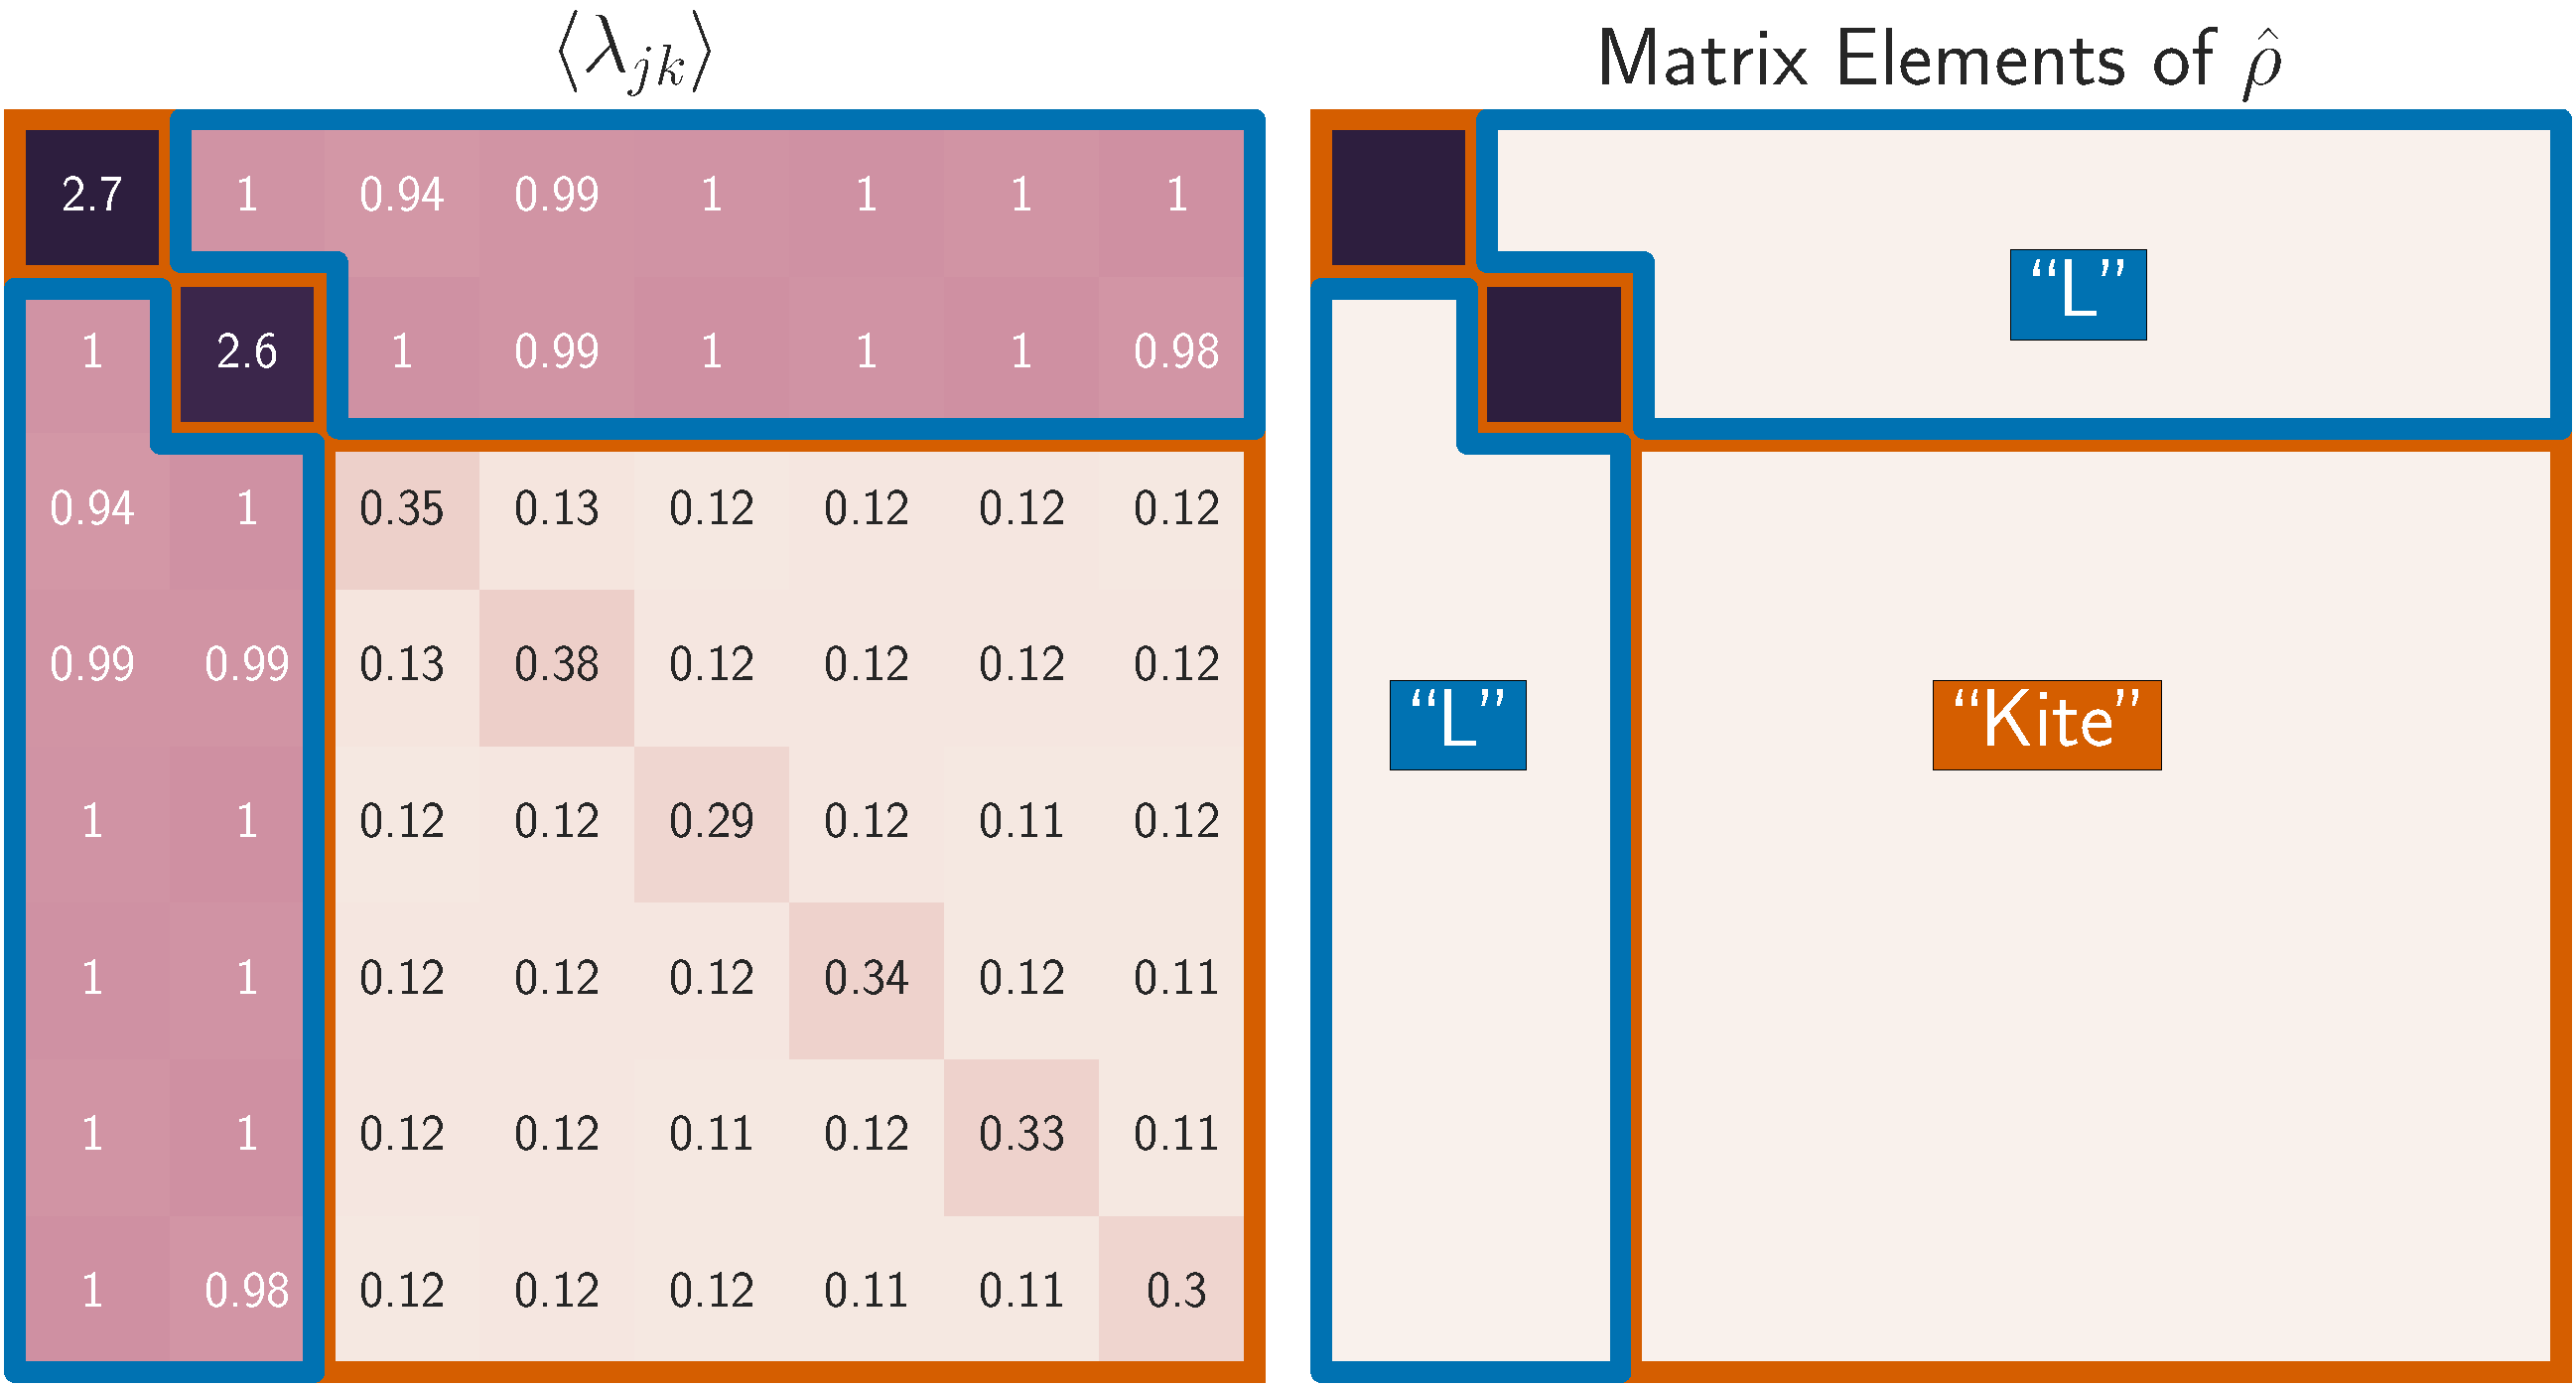
\includegraphics[width=\columnwidth]{Images/Figure_2.pdf}
 \caption{When a rank-2 state is reconstructed in $d=8$ dimensions, the total loglikelihood ratio $\lambda(\rho_0,\mathcal{M}_8)$ is the sum of terms $\lambda_{jk}$ from errors in each matrix element $(\rhoML{d})_{jk}$.  \textbf{Left}:  Numerics show a clear division; some matrix elements have $\expect{\lambda_{jk}}\sim1$ as predicted by the Wilks Theorem, while others are either more or less. \textbf{Right}:  The numerical results motivate dividing the elements of $\rhohat$ into two parts: the ``kite'' and the ``L''.}
\label{fig:L}
\end{figure}

In doing so, it is helpful to think about the error of the unconstrained estimate $\delta \equiv \hat\rho- \rho_{0}$, a normally-distributed \emph{traceless} matrix.  To simplify the analysis, we explicitly drop the $\Tr(\rho)=1$ constraint and let $\delta$ be $\mathcal{N}(0,\epsilon^2\Id)$ distributed over the $d^2$-dimensional space of Hermitian matrices (a good approximation when $d\gg2$) \footnote{That is, we let $\mathrm{Tr}(\delta)$ fluctuate as well.}, which makes $\delta$ proportional to an element of the Gaussian Unitary Ensemble (GUE) \cite{Fyodorov2005}.

\subsubsection{Computing $\langle \lambda_\mathrm{L}\rangle$}

To first order in $\epsilon$, elements of $\delta$ in the ``L'' do not affect positivity, so they are unconstrained by the boundary, and behave exactly as expected from classical theory. The $\delta_{jk}$ in the ``L'' may be seen as errors which arise due to small unitary perturbations of $\rho_{0}$. Writing $\rhohat = U^{\dagger}\rho_{0}U$, where $U=e^{i\epsilon H}$, we have
\[\rhohat \approx \rho_{0} + i\epsilon [\rho_{0},H]+\mathcal{O}(\epsilon^{2}).\]
Then, $\delta \approx i\epsilon [\rho_{0},H]$.
If $j = k$, then $\delta_{jj} = 0$. Thus, small unitaries cannot create errors in the diagonal matrix elements, at $\mathcal{O}(\epsilon)$. If $j \neq k$, then $\delta_{jk} \neq 0$, in general. (Small unitaries \emph{can} introduce errors on off-diagonal elements.)

However, if either $j$ or $k$ (or both) lie within the \emph{kernel} of $\rho_{0}$ (i.e., $\langle k | \rho_{0}| k \rangle$ or $\langle j|\rho_{0}|j\rangle$ is 0), then the corresponding $\delta_{jk}$ are zero. The only off-diagonal elements where small unitaries can introduce errors are those which are coherent between the kernel of $\rho_{0}$ and its support. These off-diagonal elements are precisely the ``L", and are  the set $\{\delta_{jk}~|~\langle j | \rho_{0}|j\rangle \neq 0, j\neq k, ~ 0 \leq j,k \leq d - 1\}$. Each $\delta_{jk}$ in the ``L'' is a $\mathcal{N}(0, \epsilon^{2})$ random variable, and crucially, is identical to the error $(\rhoML{d} - \rho_{0})_{jk}$. This is because these $\delta_{jk}$ are \emph{unaffected by the boundary}, so when we impose the positivity constraint (i.e., compute $\rhoML{d}$), their values remain the same. Therefore, $\langle \lambda_{jk}\rangle = \langle \delta_{jk}^{2}\rangle /\epsilon^{2} = 1$. As there are $2rd - r(r+1)$ of them, $\expect{\lambda_{\mathrm{L}}} = 2rd - r(r+1)$.

\subsubsection{Setting the Stage to Compute $\langle \lambda_\mathrm{kite}\rangle$}

We next need a procedure to compute $\rhoML{d}$ given $\rhohat$ -- i.e., to solve the optimization problem in Eq. \eqref{eq:mleopt}.  Fortunately, an algorithm for doing so was presented in Ref. \cite{Smolin2012}:
\begin{enumerate}[noitemsep]
\item Subtract $q\Id$ from the unconstrained $\hat\rho$, for a particular real scalar $q$,
\item ``Truncate'' $\hat\rho-q\Id$, by replacing each of its negative eigenvalues with zero.
\end{enumerate}
Here, $q$ is defined implicitly such that $\Tr\left[ \mathrm{Trunc}(\hat\rho-q\Id)\right] = 1$.

Although this was intended as a (very fast) numerical algorithm, we will manipulate it (by a series of approximations) to derive a closed-form expression for the average $\expect{\lambda}$.  

Computing $\expect{\lambda_{\mathrm{kite}}}$ is a bit harder, because the boundary \emph{does} constrain its elements.  Here, we turn to the truncation algorithm given above for finding $\rhoML{d}$, which is most naturally performed in the eigenbasis of $\hat\rho$.  Exact diagonalization of $\hat\rho$ is not feasible analytically, but only the \emph{small} eigenvalues of $\hat\rho$ are critical in truncation.  As long as all the nonzero eigenvalues of $\rho_0$ are much larger than $\epsilon$, the eigenbasis of $\hat\rho$ is accurately approximated by: (1) 
the eigenvectors of $\rho_0$ on its support; and (2) the eigenvectors of $\delta_{\mathrm{ker}} = \Pi_{\mathrm{ker}}\delta\Pi_{\mathrm{ker}}$, where $\Pi_{\mathrm{ker}}
$ is the projector onto the kernel of $\rho_0$.

Changing to this basis diagonalizes the ``kite'' portion of $\delta$, and leaves all elements of the ``L'' unchanged (at $\mathcal{O}(\epsilon)$).  The diagonal elements of $\hat\rho$ now fall into two categories:
\begin{enumerate}[noitemsep]
\item $r$ elements corresponding to the eigenvalues of $\rho_0$, which are given by $p_{j} = \rho_{jj} + \delta_{jj}$ where  $\rho_{jj}$ is the $j^{\mathrm{th}}$ eigenvalue of $\rho_{0}$, and $\delta_{jj} \sim \mathcal{N}(0,\epsilon^2)$.
\item $N \equiv d-r$ elements that are eigenvalues of $\delta_{\mathrm{ker}}$, which we denote by $\bvec{\kappa} = \{\kappa_j:~j = 1\ldots 
N\}$,
\end{enumerate}
and $\lambda_{\mathrm{kite}}$ is
\begin{equation}
\label{eq:llrs_kite}
\epsilon^{2}\lambda_{\mathrm{kite}} = \sum_{j=1}^{r}[\rho_{jj}- (p_j-q)^{+}]^2 + \sum_{j=1}^{N}\left[(\kappa_j-q)^+\right]^2,
\end{equation}
where $(x)^{+} = \max(x, 0)$. $q$ is implicitly defined such that $f(q) \equiv \Tr\left[\mathrm{Trunc}(\hat\rho - q \Id)\right]$ satisfies $f(q) = 1$. In terms of the eigenvalues of $\rhohat$, this means $q$ is the solution to
\begin{equation}
\label{eq:q_eqn}
 \sum_{j=1}^{r}(p_j - q)^{+} + \sum_{j=1}^{N}{(\kappa_j-q)^+} = 1
\end{equation}

To solve Equation \eqref{eq:q_eqn}, and derive an approximation for \eqref{eq:llrs_kite}, we need to understand the behavior of the eigenvalues of $\delta_{\mathrm{ker}}$. It is to this problem we now turn.

\subsubsection{Approximating the Eigenvalues of a GUE($N$) Matrix}
We first observe that while the $\kappa_j$ are random variables, they are not normally distributed.  Instead, because $\delta_{\mathrm{ker}}$ is proportional to a $\mathrm{GUE}(N)$ matrix, for $N\gg1$, the distribution of any eigenvalue $\kappa_{j}$
converges to a Wigner semicircle distribution \cite{Wigner1958} given by $\mathrm{Pr}(\kappa) = \frac{2}{\pi R^{2}}\sqrt{R^{2}-\kappa^{2}}$ for $|\kappa| \leq R$, with $R = 2\epsilon\sqrt{N}$.  The eigenvalues are not independent; they tend to avoid collisions (``level avoidance'' \cite{Tao2013}), 
and typically form a surprisingly regular array over the support of the Wigner semicircle.  Since our goal is to compute $\expect{\lambda_{\mathrm{kite}}}$, we can capitalize on this behavior by replacing each random sample of $\bvec{\kappa}$ with a 
\emph{typical sample} $\bar{\bvec{\kappa}}$ given by its order statistics.  These are the average values of the \emph{sorted} 
$\bvec{\kappa}$, so $\overline{\kappa}_j$ is the average value of the $j^{\mathrm{th}}$ largest value of $\bvec{\kappa}$.  Large random samples 
are usually well approximated (for many purposes) by their order statistics even when the elements of the sample are 
independent, and level avoidance makes the approximation even better. 

\begin{figure}[h!]
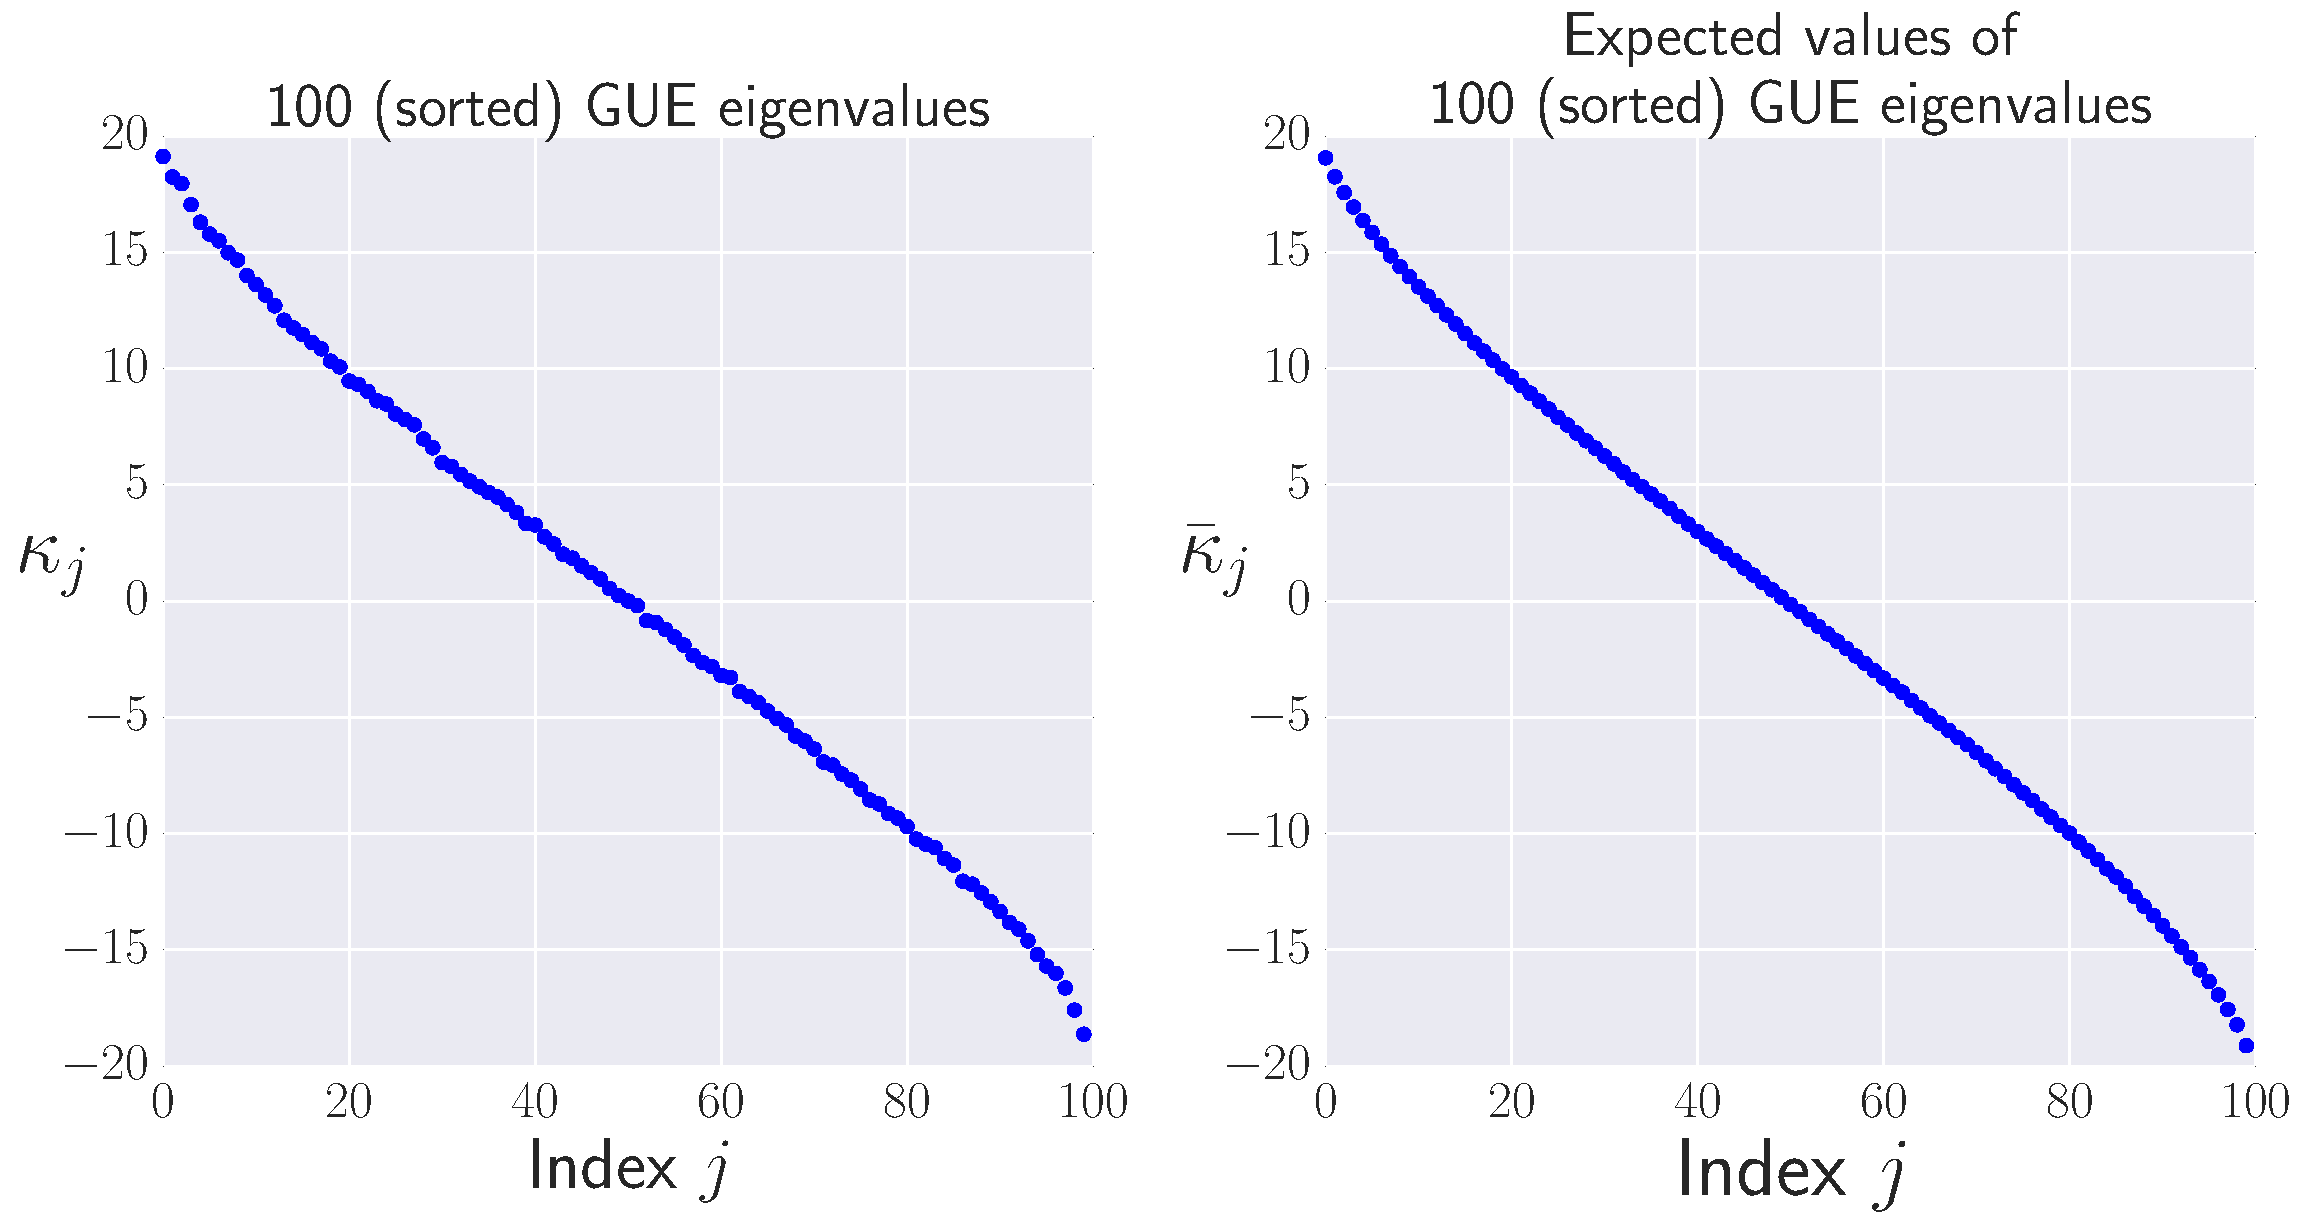
\includegraphics[width=\columnwidth]{Images/Figure_3.pdf}
\caption{Typical samples of GUE($N$) eigenvalues are accurately approximated by order statistics of the distribution (average values of a sorted sample).  \textbf{Left}:  The sorted eigenvalues (i.e., order statistics $\kappa_{j}$) of one randomly chosen GUE(100) matrix.  \textbf{Right}:  Approximate expected values of the order statistics, $\bar{\kappa}_{j}$, of the GUE(100) distribution, computed as the average of the sorted eigenvalues of 100 randomly chosen GUE(100) matrices.}
\label{fig:orderstatistics1}
\end{figure}

Suppose that $\bvec{\kappa}$ are the eigenvalues of a GUE($N$) matrix, sorted from highest to lowest.  Figure \ref{fig:orderstatistics1} illustrates such a sample for $N=100$.  It also shows the \emph{average} values of 100 such samples (all sorted).  These are the \emph{order statistics} $\overline{\bvec{\kappa}}$ of the distribution (more precisely, what is shown is a good \emph{estimate} of the order statistics; the actual order statistics would be given by the average over infinitely many samples).  The point of the figure is to show that, while the order statistics \emph{are} slightly more smoothly and predictably distributed than a single (sorted) sample, the two are remarkably similar.  A single sample $\bvec{\kappa}$ will fluctuate around the order statistics, but these fluctuations are relatively small, partly because the sample is large, and partly because the GUE eigenvalues experience level repulsion.  Thus, the ``typical'' behavior of a sample -- by which we mean the mean value of a statistic of the sample -- is well captured by the order statistics (which have no fluctuations at all).

We now turn to the problem of modeling $\bvec{\kappa}$ quantitatively.  We note up front that we are only going to be interested in certain properties of $\bvec{\kappa}$:  specifically, partial sums of all $\kappa_j$ greater or less than the threshold $q$, or partial sums of functions of the $\kappa_j$ (e.g. $(\kappa_j-q)^2$).  We require only that an ansatz be accurate for such quantities.  We do not use this fact explicitly, but it motivates our approach -- and we do not claim that our ansatz is accurate for \emph{all} conceivable functions.

In general, if a sample $\bvec{\kappa}$ of size $N$ is drawn so that each $\kappa$ has the same probability density 
function $\mathrm{Pr}(\kappa)$, then a good approximation for the $j^{\mathrm{th}}$ order statistic is given by the inverse 
\emph{cumulative} distribution function (CDF):
\begin{equation}
\overline{\kappa}_j \approx \mathrm{CDF}^{-1}\left(\frac{j-1/2}{N}\right).
\end{equation}
This is closely related to the observation that the histogram of a sample tends to look similar to the underlying probability density function.  More precisely, it is equivalent to the observation that the empirical distribution function (the CDF of the histogram) tends to be (even more) similar to the underlying CDF.  (For i.i.d. samples, this is the content of the Glivenko-Cantelli theorem \cite{VanderVaart2000}).  Figure \ref{fig:orderstatistics2} compares the order statistics of GUE(100) and GUE(10) eigenvalues (computed as numerical averages over 100 random samples) to the inverse CDF for the Wigner semicircle distribution.  Even though the Wigner semicircle model of GUE eigenvalues is only exact as $N\to\infty$, it provides a nearly-perfect model for $\overline{\bvec{\kappa}}$ even at $N=10$ (and remains surprisingly good all the way down to $N=2$).

\begin{figure}[h!]
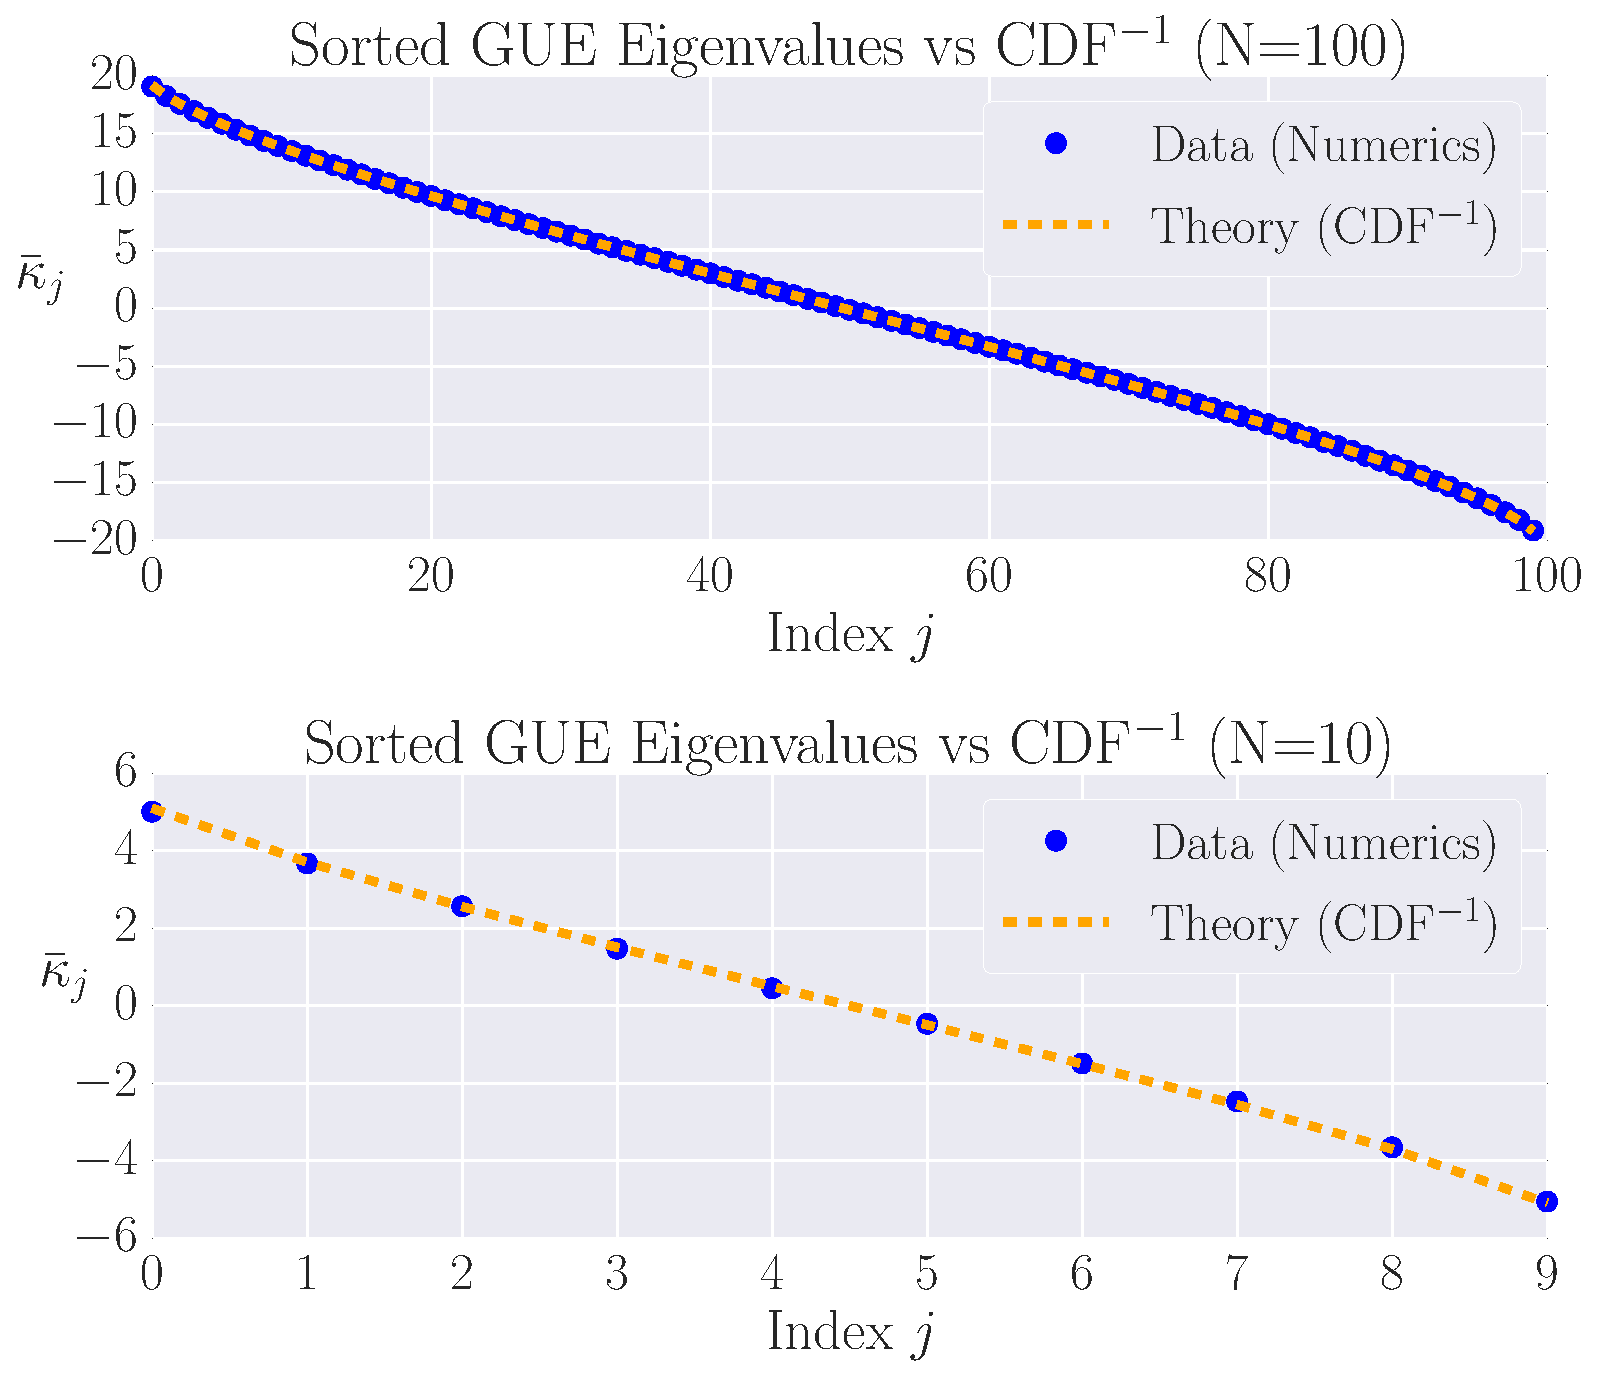
\includegraphics[width=\columnwidth]{Images/Figure_4.pdf}
\caption{Order statistics of the GUE($N$) eigenvalue distribution are very well approximated by the inverse CDF of the Wigner semicircle distribution.  In both figures, we compare the order statistics of a GUE($N$) distribution to the inverse CDF of the Wigner semicircle distribution. \textbf{Top}:  $N=100$.  \textbf{Bottom}:  $N=10$.
Agreement in both cases is essentially perfect.}
\label{fig:orderstatistics2}
\end{figure}

We make one further approximation, by assuming that $N\gg1$, so the distribution of the $\overline{\kappa}_j$ is effectively continuous and identical to $\mathrm{Pr}(\kappa)$. For the quantities that we compute, this is equivalent to replacing the empirical distribution function (which is a step function) by the CDF of the Wigner semicircle distribution.  So, whereas for any given sample the partial sum of all $\kappa_j > q$ jumps discontinuously when $q=\kappa_j$ for any $j$, in this approximation it changes smoothly.  This accurately models the \emph{average} behavior of partial sums.

\subsubsection{Deriving an Approximation for $q$}
The approximations of the previous section allow us to use the following ansatz for the eigenvalues of $\hat\rho$; namely, $\{p_j\} \cup \{\overline{\kappa}_j\}$, where the $p_j$ are $\mathcal{N}(\rho_{jj},\epsilon^2)$ random variables, and the $\overline{\kappa}_j$ are the (fixed, smoothed) order statistics of a Wigner semicircle distribution.  In turn, the defining equation for $q$ (Equation \eqref{eq:q_eqn}) is well approximated as
\begin{equation}
\sum_{j=1}^{r}(p_j - q)^{+} + \sum_{j=1}^{N}{(\overline{\kappa}_j-q)^+} \approx 1
\end{equation}
To solve this equation, we observe that the $\overline{\kappa}_j$ are symmetrically distributed around $
\kappa=0$, so half of them are negative.  Therefore, with high probability, $\Tr
\left[\mathrm{Trunc}(\hat\rho)\right]>1$, and so we will need to subtract $q\Id$ from $\hat\rho$ before truncating. (This is in distinction to the case where we have to \emph{add} $q$.)

We make another assumption; namely, that the eigenvalues of $\rho_{0}$ are large compared to the perturbations $\delta_{jj}$ and $q$. This implies $(p_{j} - q)^{+} = p_{j} - q$. Under this assumption, $q$ is the solution to
\begin{align}
\nonumber 1 &\approx \sum_{j=1}^{r}(p_j - q)^{+} + \sum_{j=1}^{N}{(\overline{\kappa}_j-q)^+}\\
\nonumber &\approx 1 - rq + \Delta + N\int_{\kappa=q}^{2\epsilon\sqrt{N}}{(\kappa-q)\mathrm{Pr}(\kappa)\mathrm{d}\kappa}\\
\label{eq:q_eqn2}\implies 0 &= - rq + \Delta + \frac{\epsilon}{12\pi}\left[
\begin{array}{l} (q^2+8N)\sqrt{-q^2+4N} \\
-12qN\left(\frac{\pi}{2}-\sin^{-1}\left(\frac{q}{2\sqrt{N}}\right)\right)
\end{array}\right],\nonumber\\
~
\end{align}
where $\Delta = \sum_{j=1}^{r}\delta_{jj}$ is a $\mathcal{N}(0,r\epsilon^2)$ random variable.  We choose to replace a discrete 
sum (line 1) with an integral (line 2). This approximation is valid when $N\gg1$, as we can accurately approximate a discrete collection of closely spaced real numbers by a smooth density or distribution over the real numbers that has approximately the same CDF.  It is also remarkably accurate in practice.
  
In yet another approximation, we replace $\Delta$ with its average value, which is zero.  We could obtain an even more accurate expression 
 by treating the fluctuations in $\Delta$ more carefully, but this crude approximation turns out to be quite accurate already.

To solve Equation \eqref{eq:q_eqn2}, it is necessary to further simplify the complicated expression resulting from the integral (line 3).  To do so, we 
assume  $\rho_0$ is relatively low-rank, so $r \ll N$.  In this case, the sum of the positive $\overline{\kappa}_j$ is large compared 
with $r$, almost all of them need to be subtracted away, and therefore $q$ is close to $2\epsilon\sqrt{N}$.  \footnote{This justifies the assumption that $\rho_{jj} + \delta_{jj} - q > 0$.} We therefore replace 
the complicated expression with its leading order Taylor expansion around $q=2\epsilon\sqrt{N}$, substitute into Equation \eqref{eq:q_eqn2}, and 
obtain the equation
\begin{equation}
\frac{rq}{\epsilon}  = \frac{4}{15\pi}N^{1/4}\left(2\sqrt{N}-\frac{q}{\epsilon}\right)^{5/2}.
\end{equation}
This equation is a quintic polynomial, so it has no closed-form solution.  However, its roots have a well-defined asymptotic ($N\to
\infty$) expansion that becomes accurate quite rapidly (e.g., for $N>4$):
\begin{equation}
\label{eq:truncation}
z \equiv q/\epsilon \approx 2\sqrt{N}-\frac{(240r\pi)^{2/5}}{4}N^{1/10}+\frac{(240r\pi)^{4/5}}{80}N^{-3/10}.
\end{equation}

\todo[inline]{Do we want a figure of how well this does?}

\subsubsection{Computing $\langle \lambda_{\mathrm{kite}}\rangle$}
Now that we know how much to subtract off in the truncation process, we can approximate $\expect{\lambda_{\mathrm{kite}}}$, originally given in Equation \eqref{eq:llrs_kite}:
\begin{align}
\nonumber \expect{\lambda_{\mathrm{kite}}} &\approx  \frac{1}{\epsilon^{2}}\left\langle\sum_{j=1}^{r}[\rho_{jj}- (p_j-q)^{+}]^2 + \sum_{j=1}^{N}\left[(\bar{\kappa}_j-q)^+\right]^2 \right\rangle\\
\nonumber &\approx \frac{1}{\epsilon^{2}} \left\langle\sum_{j=1}^{r}[-\delta_{jj} +  q ]^2 + \sum_{j=1}^{N}\left[(\bar{\kappa}_j-q)^+\right]^2 \right\rangle\\
\nonumber  &\approx r + rz^2 + \frac{N}{\epsilon^{2}}\int_{\kappa=q}^{2\epsilon\sqrt{N}}{ \mathrm{Pr}(\kappa)(\kappa-q)^2 d\kappa} \\
\nonumber &=r + rz^{2} + \frac{N(N+z^{2})}{\pi}\left(\frac{\pi}{2} - \sin^{-1}\left(\frac{z}{2\sqrt{N}}\right)\right) \\
& - \frac{z(z^{2}+26N)}{24\pi}\sqrt{4N-z^{2}}
\end{align}

\section{Result for $\langle \lambda \rangle$, Comparison to Numerical Experiments}
The total expected value, $\expect{\lambda} = \expect{\lambda_{\mathrm{L}}} + \expect{\lambda_{\mathrm{kite}}}$, is thus
\begin{align}
\label{eq:ourLLRS}
\nonumber \langle \lambda(\rho_{0}, \M_{d}) \rangle &\approx 2rd - r^{2}+rz^{2}\\
\nonumber & + \frac{N(N+z^{2})}{\pi}\left(\frac{\pi}{2} - \sin^{-1}\left(\frac{z}{2\sqrt{N}}\right)\right) \\
& - \frac{z(z^{2}+26N)}{24\pi}\sqrt{4N-z^{2}}
\end{align}
where $z$ is given in Equation \eqref{eq:truncation}, $N=d-r$, and $r = \mathrm{Rank}(\rho_{0})$.

Equation \eqref{eq:ourLLRS} is our main result.  To test its validity, we compare it to numerical simulations for $d=2,\ldots,30$ and $r=1,\ldots,10$, in Figure \ref{fig:modelcomp-iso}.  The prediction of the Wilks theorem is wildly incorrect for $r\ll d$. In contrast, Equation \eqref{eq:ourLLRS} is almost perfectly accurate when $r \ll d$, but it does begin to break down (albeit fairly gracefully) as $r$ becomes comparable to $d$.  We conclude that our analysis (and Equation \eqref{eq:ourLLRS}) correctly models tomography \emph{if} the Fisher information is isotropic ($\Fi \propto \Id$).

\begin{figure}[h]
 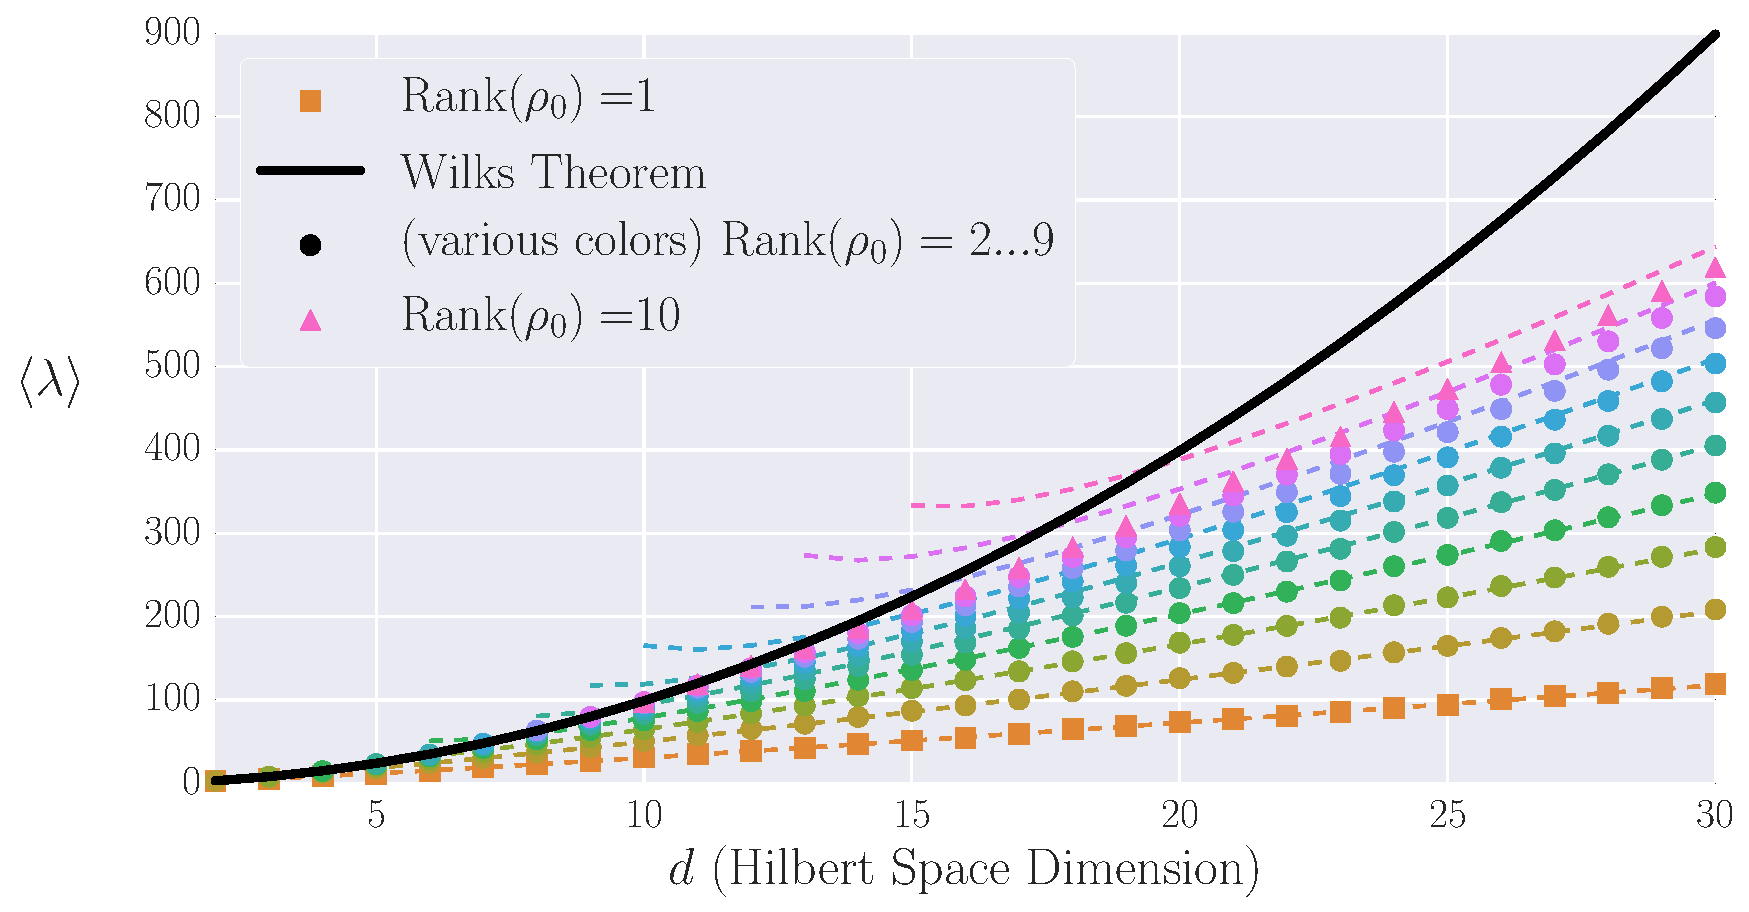
\includegraphics[width=\columnwidth]{Images/Figure_5.pdf}
 \caption{Numerical results for $\expect{\lambda}$ compared to the prediction of the Wilks theorem (solid line) and our replacement theory as given in Equation \eqref{eq:ourLLRS}, (dashed lines).  Our formula depends on the rank $r$ of $\rho_0$ (unlike the Wilks prediction), and is nearly perfect for $r\ll d$.  It becomes less accurate as $r$ approaches $d/2$, and is invalid when $r\approx d$.}
 \label{fig:modelcomp-iso}
\end{figure}

\section{Comparison to Heterodyne Tomography}
In practice, the Fisher information is rarely isotropic.  So we tested our idealized result by applying it to a realistic, challenging, and experimentally relevant problem: quantum heterodyne (equivalent to double homodyne) state tomography \cite{Lvovsky2001a, Bertrand1987, Leonhardt1995, Lvovsky2009} of a single optical mode.  (See Figure \ref{fig:fish_condition} for a plot of the \emph{condition number} -- the ratio of the largest to smallest eigenvalue -- of the estimated Fisher information. It is clear that, for such a tomographic setup, $\mathcal{I} \not \propto \Id$.) States of this continuous-variable system are described by density operators on the infinite-dimensional Hilbert space $L^2(\reals)$.  Fitting these infinitely many parameters to finitely much data demands simpler models.

We consider a family of nested models motivated by a low-energy (few-photon) ansatz, and choose   
the Hilbert space $\mathcal{H}_d$ to be that spanned by the photon number states $\{\ket{0},\ldots ,\ket{d-1}\}$.
Heterodyne tomography reconstructs $\rho_{0}$ using data from repeated measurements of the 
coherent-state POVM, $\{|\alpha\rangle\langle \alpha| /\pi, ~\alpha=x+ip\in \mathbb{C}\}$, which corresponds to sampling directly from the 
state's Husimi $Q$-function \cite{Husimi1940}.

\begin{figure}[h]
  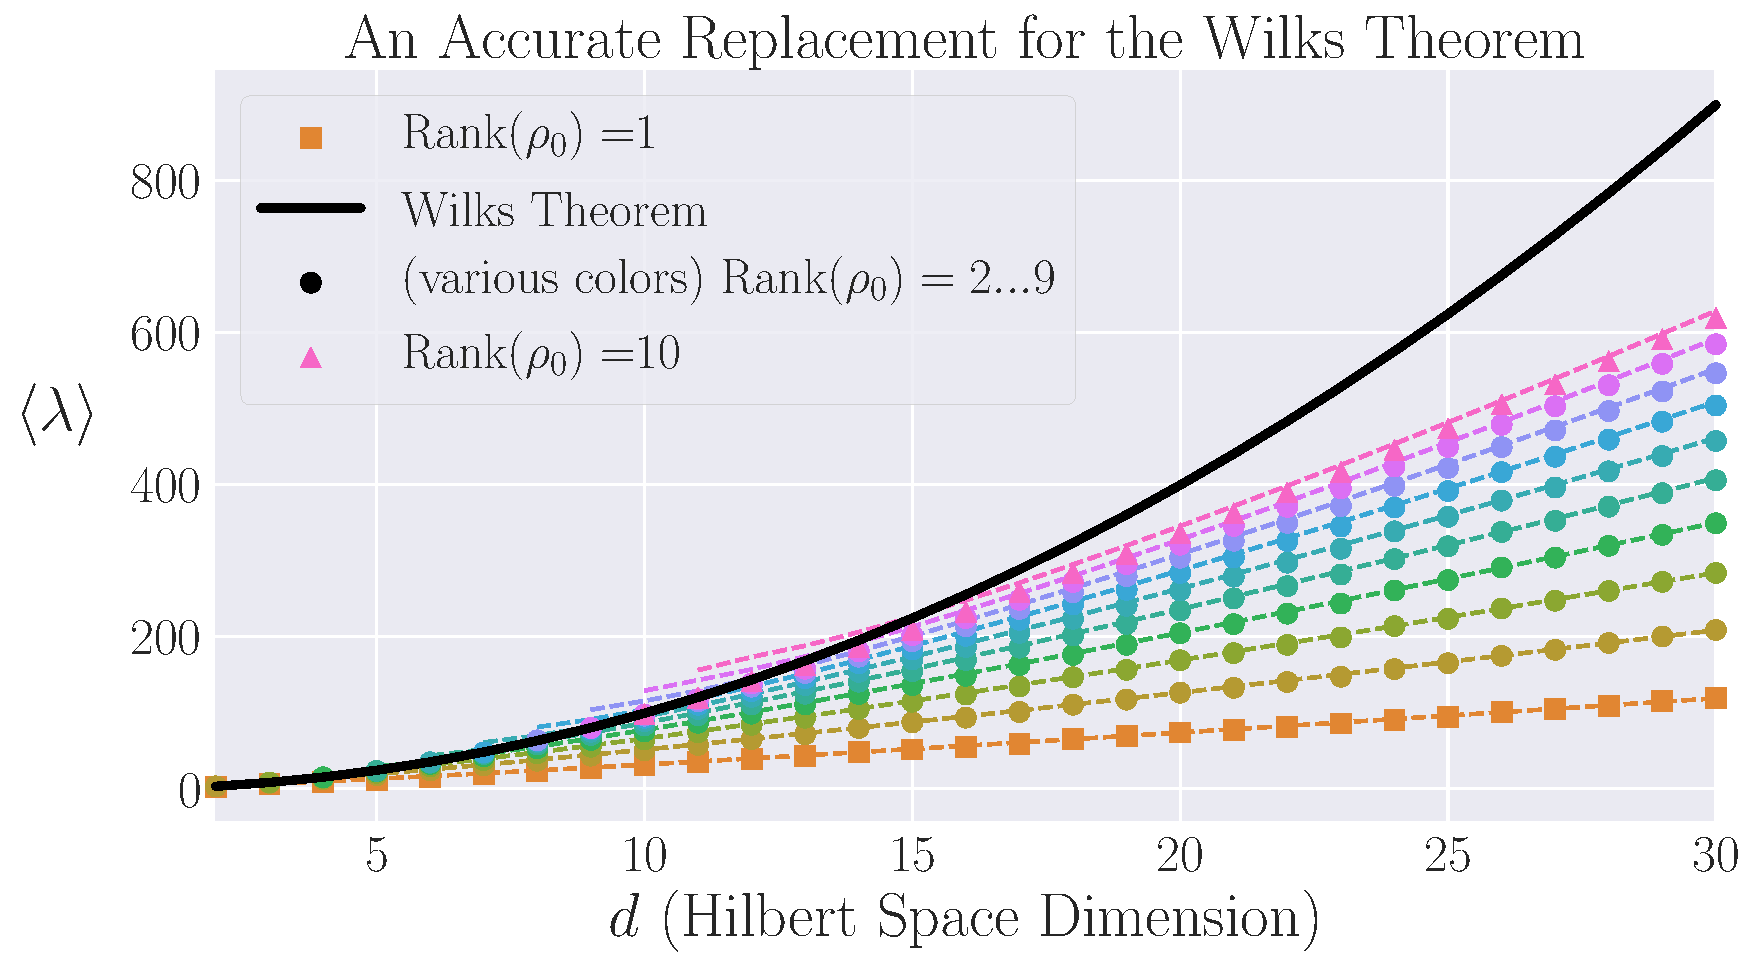
\includegraphics[width=\columnwidth]{Images/Figure_6.pdf}
 \caption{The condition number $\kappa$ -- the ratio of the largest to smallest eigenvalue -- of the estimated heterodyne Fisher information grows with model dimension, indicating an increase in anisotropy. (Estimates are the average over 100 Hessians of the loglikelihood function.) The dashed lines indicate different states $\rho_{0}$, and the solid line is $\kappa = 1$ (i.e., $\mathcal{I} \propto \Id$.).}
\label{fig:fish_condition}
\end{figure}

We examined the behavior of $\lambda$ for 13 distinct states $\rho_{0}$, both pure and mixed, supported on $\mathcal{H}_{2}, \mathcal{H}_{3}, \mathcal{H}
_{4}$, and $\mathcal{H}_{5}$.  We used rejection sampling to simulate 100 heterodyne datasets with up to $N_{\mathrm{samples}}=10^5$, and found MLEs over each of the 9 models $\M_2, \ldots, M_{10}$ using numerical optimization \footnote{The model $\M_{1}$ is trivial, as $\M_{1} = \{|0\rangle \langle 0|\}$. This model will almost always be wrong, in general.}.  For each $\rho_{0}$ and each $d$, we averaged $\lambda(\rho_{0}, \M_{d})$ over all 100 datasets to obtain an empirical average loglikelihood ratio $\bar{\lambda}$ for each $(\rho_0,d)$ pair.

\begin{figure}[h]
 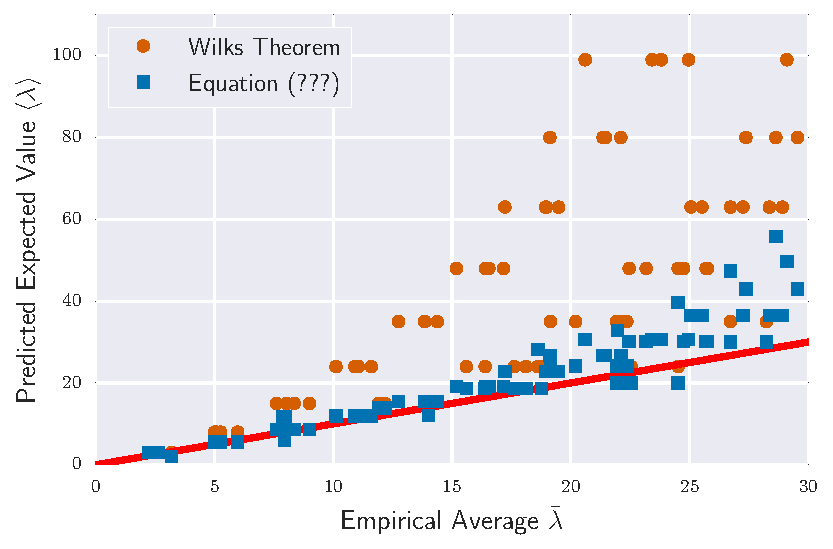
\includegraphics[width=\columnwidth]{Images/Figure_7.pdf}
 \caption{The Wilks theorem (orange dots) dramatically over-estimates $\langle\lambda(\rho_{0}, \M_{d})\rangle$ in optical heterodyne tomography. Our formula, Equation \ref{eq:ourLLRS} (blue squares), is far more accurate. Residual discrepancies occur in large part because $N_{\mathrm{samples}}$ is not yet ``asymptotically large''. The solid red line corresponds to perfect correlation between theory ($\expect{\lambda}$) and practice ($\bar\lambda$).}
 \label{fig:modelcomp}
\end{figure}

Results of this test are shown in Figure \ref{fig:modelcomp}, where we plot the predictions for $\langle \lambda \rangle$ given by the Wilks theorem and Equation \eqref{eq:ourLLRS}, against the empirical average $\bar\lambda$, for a variety of $\rho_{0}$ and $d$. Our formula correlates very well with the empirical average, while the Wilks theorem (unsurprisingly) overestimates $\lambda$ dramatically for low-rank states.  Whereas a model selection procedure based on Wilks theorem would tend to falsely reject larger Hilbert spaces (by setting the threshold for acceptance too high), our formula provides a reliable null theory.

Interestingly, as $d$ grows, Equation \eqref{eq:ourLLRS} also begins to overpredict. As Figure \ref{fig:totalcontrib} indicates, a more accurate description is that the numerical experiments are \emph{underachieving}, because $\bar\lambda$ is still growing with $N_{\mathrm{samples}}$.  Both the Wilks theorem and our analysis are derived in an asymptotic limit $N \rightarrow \infty$; for finite but large $N$, both may be invalid.  Figure \ref{fig:totalcontrib} shows that, even at $N\sim 10^{5}$, the behavior of $\bar{\lambda}$ has failed to become asymptotic. This is surprising, and suggests heterodyne tomography is a particularly exceptional and challenging case to model statistically. 

\begin{figure}[h]
  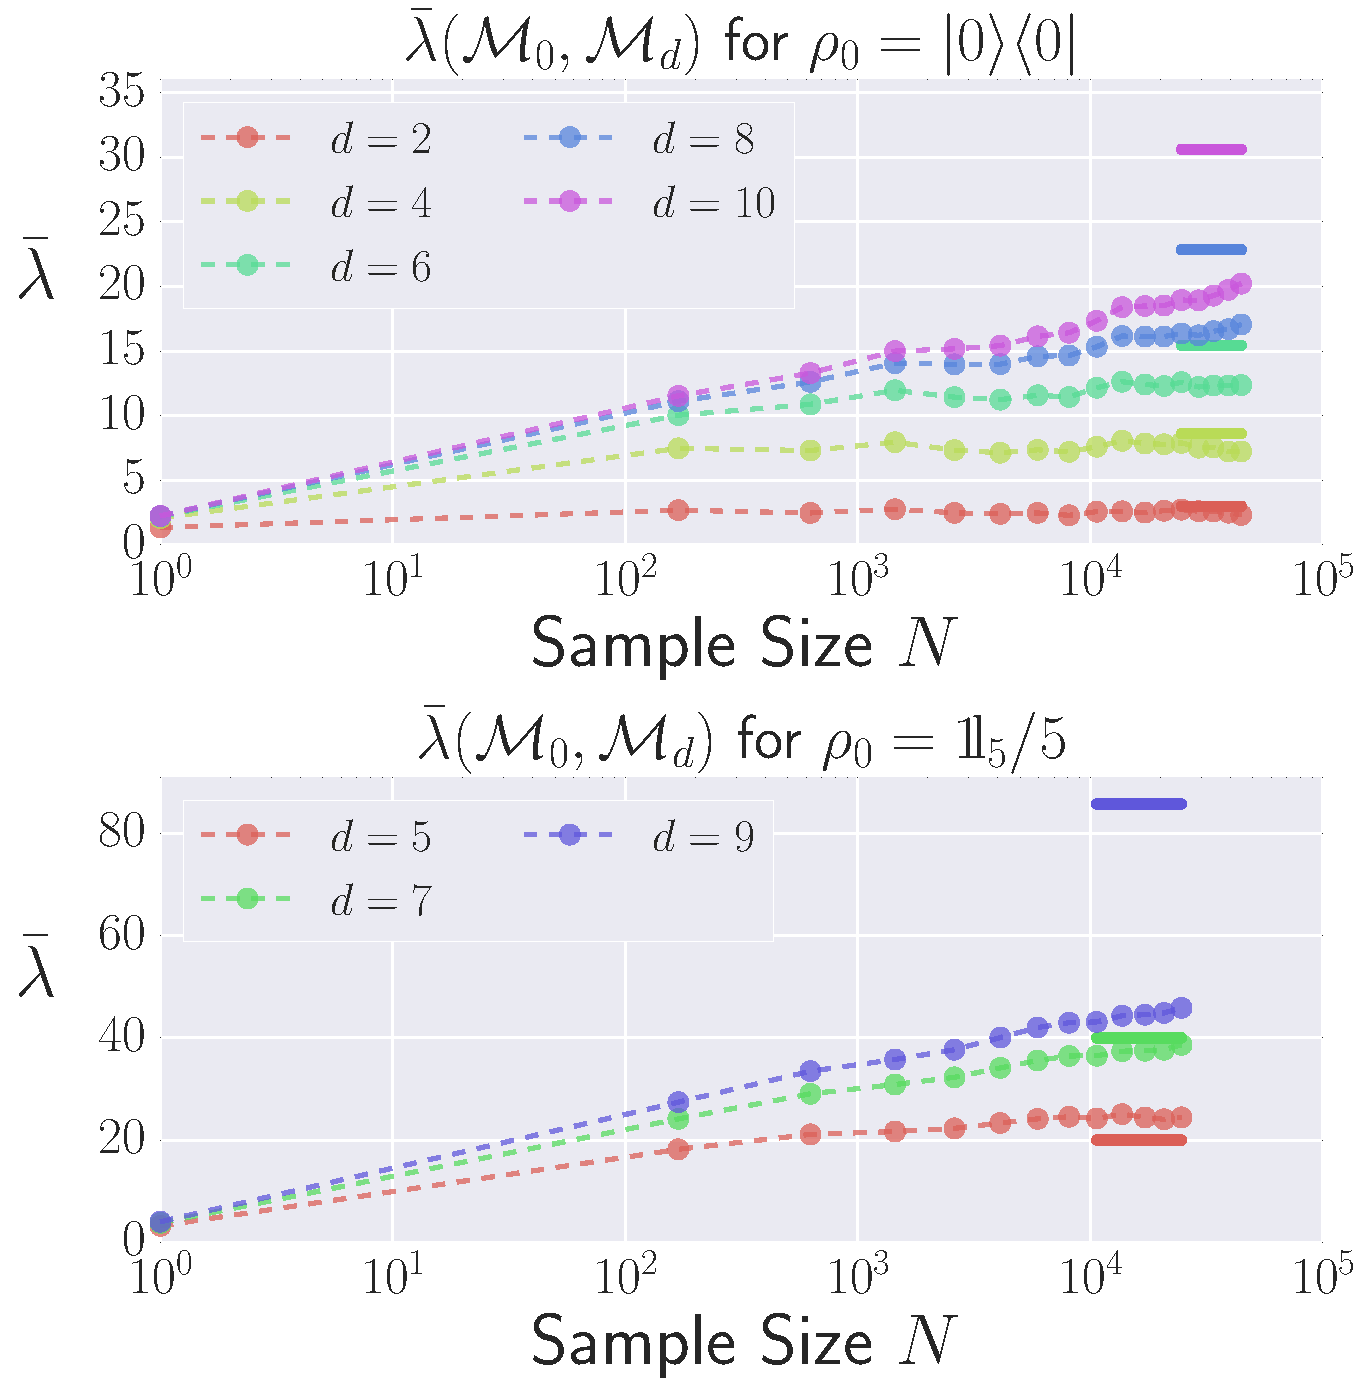
\includegraphics[width=\columnwidth]{Images/Figure_8.pdf}
 \caption{The empirical average $\bar{\lambda}$  may have achieved its asymptotic value, or is still 
growing, depending on the true state $\rho_{0}$ and the model dimension $d$. Solid lines indicate the value of our formula
for the asymptotic expected value, given in Equation \eqref{eq:ourLLRS}.}
\label{fig:totalcontrib}
\end{figure}


However, our model \emph{does} get some of the qualitative features correct. In Figure \ref{fig:model_comparison}, we look at $\langle \lambda_{jk}\rangle$, where we assume an isotropic Fisher information, and when we simulate heterodyne tomography. While the numbers given for $\langle \lambda_{jk} \rangle$ do not agree exactly, they still break down into two groups, the ``L" and the ``kite". (See Figure \ref{fig:individcontrib} for an analysis of the exact differences in the values.)
 
 
\begin{figure}[h]
  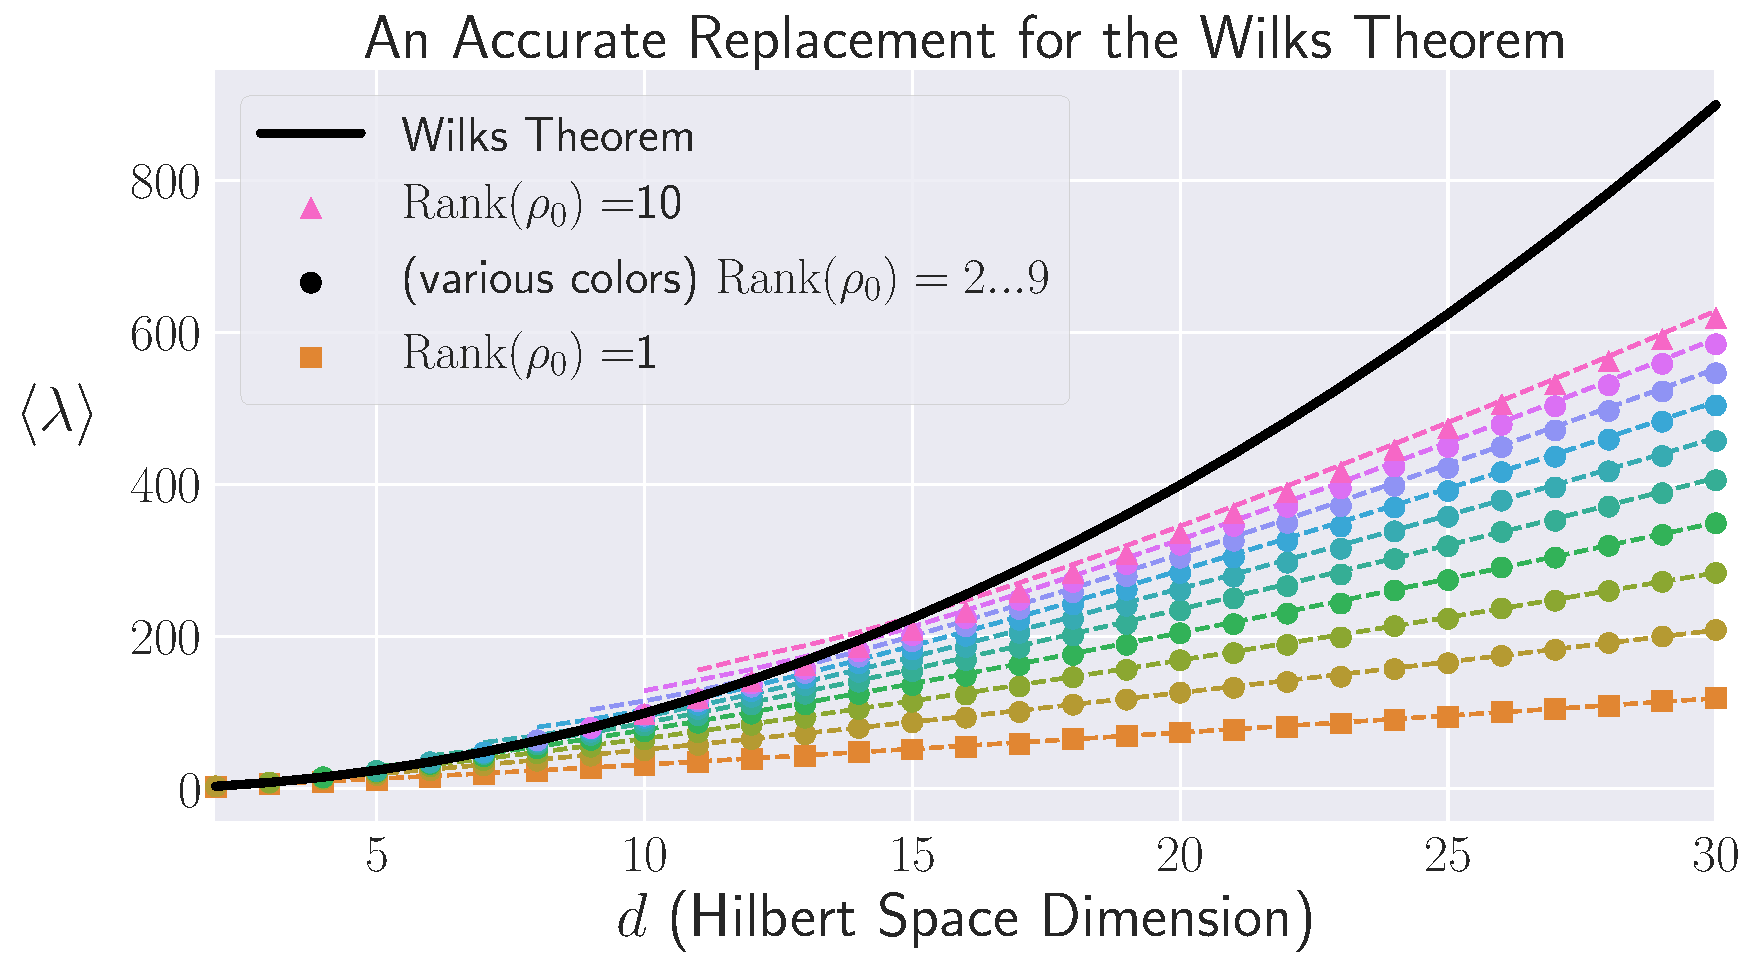
\includegraphics[width=\columnwidth]{Images/Figure_9.pdf}
 \caption{The values of $\langle \lambda_{jk} \rangle$ assuming an isotropic Fisher information (left), and for heterodyne tomography (right). \textbf{Top}: $\rho_{0} = |0\rangle\langle 0|$. \textbf{Bottom}: $\rho_{0} = \mathcal{I}_{2}/2$. \textbf{Discussion}: Qualitatively, the behavior is the same, though there are quantitative differences, particularly within the kite.}
\label{fig:model_comparison}
\end{figure}

\begin{figure}[h]
  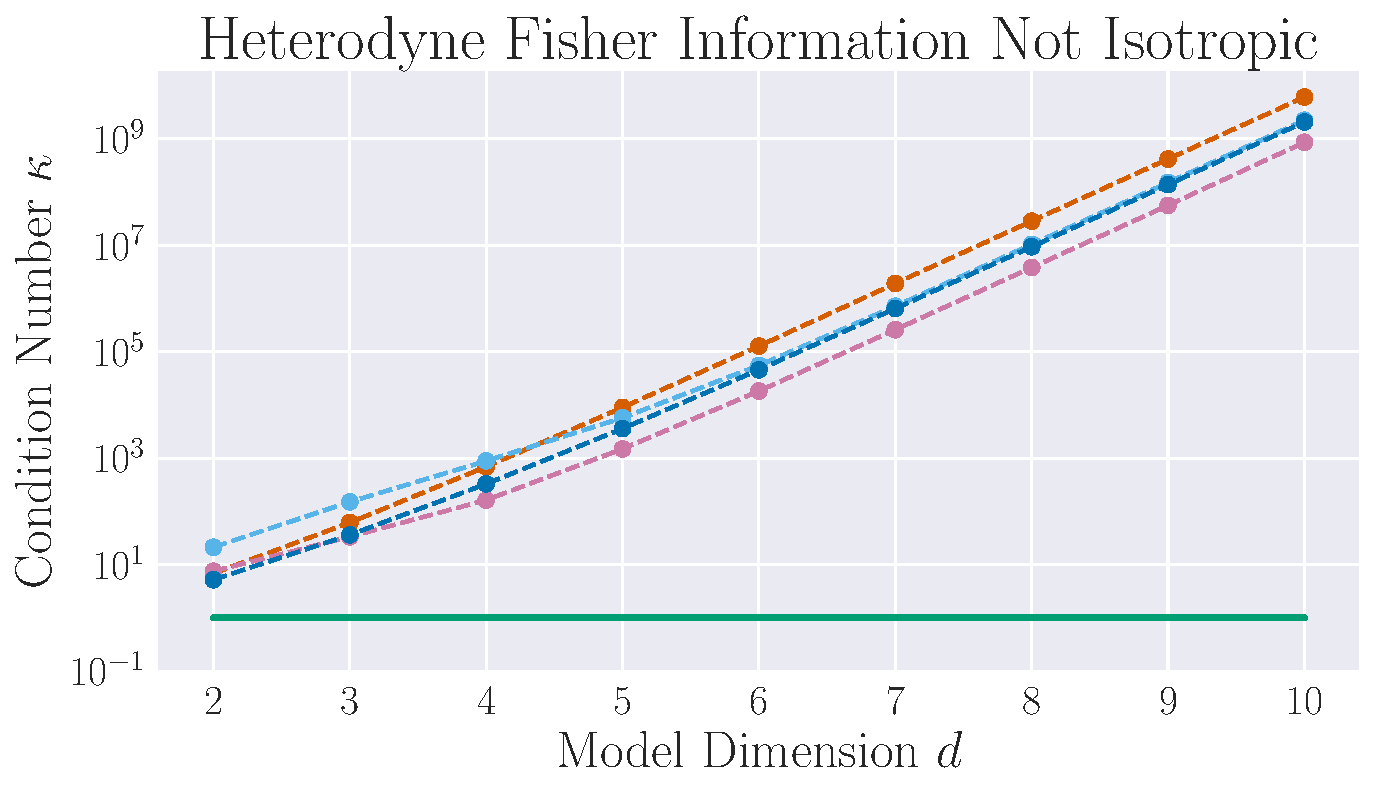
\includegraphics[width=\columnwidth]{Images/Figure_10.pdf}
 \caption{Examining how our predicted values for $\langle \lambda_{jk} \rangle$ disagree with simulated heterodyne experiments. We take $\rho_{0} = |0\rangle\langle 0|$ and $d=8$. \textbf{Top Left}: The values of  $\langle \lambda_{0k}\rangle$ in the ``L" as a function of sample size $N$.  \textbf{Top Right}:  Even at the largest $N$ studied, $\langle \lambda_{0k}\rangle$ is nontrivially less than 1, especially for the higher number states. \textbf{Bottom Left}: The total from the ``kite" versus $N$. It is clear the total is still growing. \textbf{Bottom Right}: The individual ``kite" elements $\langle \lambda_{jk}\rangle$ at the largest $N$ studied;  most are small compared to values they would have in the isotropic case.}
\label{fig:individcontrib}
\end{figure}



\section{Conclusions and Discussion}
The Wilks theorem is not generally reliable in quantum state tomography, but our Equation \eqref{eq:ourLLRS} provides a much more broadly applicable replacement that can be used in model selection methods.  This includes protocols like the AIC and BIC \cite{Akaike1974, Schwarz1978, Kass1995, Burnham2004} that do not explicitly use the Wilks theorem, but rely on the same assumptions (asymptotic normality, etc).  Null theories of loglikelihood ratios have many other applications, including hypothesis testing \cite{Blume-Kohout2010,Moroder2013} and confidence regions \cite{Glancy2012a}, and our result is directly applicable to them.  Refs. \cite{Moroder2013,Glancy2012a} both point out explicitly that their methods are unreliable near boundaries and therefore cannot be applied to rank-deficient states; our result fixes this outstanding problem.  However, our numerical experiments with heterodyne tomography show unexpected behavior, indicating that quantum tomography can still surprise, and may violate \emph{all} asymptotic statistics results.  In such cases, bootstrapping \cite{Efron1979, Higgins2004} may be the only reliable way to construct null theories for $\lambda$.  Finally, the \emph{methods} presented here have application beyond the analysis of loglikelihoods.  They shed light on the behavior of $\rhoML{d}$ for rank-deficient states, and can be used to predict other derived properties such as the average rank of the estimate, which is independently interesting for (e.g.) quantum compressed sensing \cite{Flammia2012a, Steffens2016, Kalev2015, Kalev2015a}.

\section{Acknowledgements:} The authors are grateful for those who provide support for the following software packages: iPython/Jupyter \cite{Perez}, matplotlib
\cite{Hunter2007}, mpi4py \cite{Dalcin2011},  NumPy \cite{VanDerWalt2011}, pandas \cite{mckinney2010}, Python 2.7 
\cite{vanRossum}, seaborn \cite{Waskom2016}, and SciPy \cite{Oliphant2007a}. TLS thanks Jonathan A Gross for helpful 
discussions on software design, coding, and statistics, John King Gamble for useful insights on parallelized 
computation and feedback on earlier drafts of this paper, and Daniel Seuss for proofreading edits.

Sandia National Laboratories is a multi-mission laboratory managed and operated by National Technology and Engineering Solutions of Sandia, LLC., a wholly owned subsidiary of Honeywell International, Inc., for the U.S. Department of Energy's National Nuclear Security Administration under contract DE-NA-0003525.

\bibliographystyle{apsrev4-1}
\bibliography{wilkspaper}
\end{document}
